% !TEX encoding = UTF-8 Unicode
\documentclass[a4j,11pt,report]{jsbook}
\usepackage[dvipdfmx]{graphicx}
\usepackage{tabularx}
\usepackage{fancybox}
\usepackage{ascmac}
\usepackage{amsmath,amssymb,amsthm}
\usepackage{bm}
\usepackage{bmpsize}
\usepackage{here}
\usepackage{scalefnt}
\usepackage{moreverb}
\usepackage{multicol}
\bibliographystyle{ipsjsort}

\setlength{\topmargin}{-1in}
\addtolength{\topmargin}{5mm}
\setlength{\headheight}{5mm}
\setlength{\headsep}{0mm}
\setlength{\textheight}{\paperheight}
\addtolength{\textheight}{-25mm}
\setlength{\footskip}{5mm}

\newcommand{\frontpage}[3]{%
\title{卒業論文\\ \vspace{3em}\\{\huge #1}\\ \\#2\vspace{15em}}%
\author{{\huge 成蹊大学理工学部情報科学科}\\ \\{\huge #3}}%
\date{}
\maketitle

\thispagestyle{empty}


}


\newcommand{\point}[1]{
\begin{itembox}[l]{ポイント}
  #1
\end{itembox}
}

\begin{document}

\frontpage  % 以下の各項目を自分のテーマにあわせて修正する.
{計算問題の特徴分布にもとづく類題選出による\\自己学習支援}
{Self Learning Support by Automatic Selection of Calculation Exercises based on Feature Distribution of Exercises}
{S152114 宮地 雄也}



\chapter*{要旨}
\thispagestyle{empty}

本研究は自然言語処理の技術を人工言語の数式に適用し,適切な数式の分類ができるかどうか調べることを目的としている.提案手法では分散表現で文字の特徴量を抽出したのちその特徴量を用いて,さらに再帰ニューラルネットワークを用いて式のベクトルを得た.

提案手法を計算問題の復習を行う際の類題選出に利用し,生徒が間違えた問題の式に近い特徴をもつ式を選べることができるのを確認することができた.

現在主流なアダプティブラーニングの手法が大量の学習データを必要とするのに対して,本研究の成果を用いることで数式データのみで最適問題を選ぶことができ,復習に最適な類題選出を実現可能である.


\tableofcontents
\thispagestyle{empty}

\thispagestyle{plain}
\setcounter{page}{1}

\chapter{序論 \label{ch:introduction}}

昨今,小・中学生の理系離れが問題視されている.平成30年度全国学力・学習状況調査(全国学力テスト)(文献\cite{result_zennkoku_test})の結果では平均正答率は小学校では算数Bが51.7\%,中学校では数学が47.6\%とどちらも最も低く,ついで国語,理科の順で正答率が低い.
小中どちらとも理系教科の習熟度が低いことを示している.
全国学力テストの中に小学校6年生時に算数が好きな生徒は65.1\%に対して3年後の中学校3年生の時でも数学が好きな割合が51.6\%と低く,勉強が進むにつれ苦手な子が増えることが分かる.

この要因の一つに,数学は一つの計算方法が様々な分野に横断していくため,一度,苦手を生んでしまったらそこからの分野の理解度が下がり,次の分野での応用がきかないために連鎖的に苦手が蓄積してしまうことがあげられる.この状況を打破するには子供一人一人の苦手と向き合い,苦手と感じる前に理解していくしかない.
しかしながら,生徒と向き合うべき教師の労働時間は過酷を極めている.ベネッセ教育総合研究所の調査によると小中高の教員の領導時間は増加の一途を辿っていることを明らかにした.
表\ref{tb:teacher_time}は文献\cite{benesse_DateBook}での調査の結果の抜粋である.

表\ref{tb:teacher_time}によると,教員の労働時間は2010年に比べて2016年の方が各年次とも増加しており,教員のやることが増えている一方で,主であるはずの教材研究や教務準備に時間が割けていないことがわかる.
この状況では先生が生徒一人一人に時間をさき,指導することは難しい.

この打開策として,IT技術駆使した個人別最適化学習に注目が集まっている.
しかし,教育の情報は,生徒の情報と結びついている個人情報なためオープン化できない.
現在でているサービスでは各サービス利用者の利用状況からデータを取得し,その運用に利用しており一部の大手企業が情報を独占している.

そこで個人のデータではなく,解く数式の方に着目し,生徒が間違えた問題と同様の特徴を持つ問題が復習する類題として最適なのではないかという仮定のもと,本論文では数式の特徴を掴むために自然言語処理の分野で使用される分散表現を適用し,さらに再帰ニューラルネットワークを用いて数式ベクトルを作り出し,そのベクトルを用いて実際に復習問題選出を行う手法を提案する.

数式自体も自然言語と同様にある一定のルールがあり,自然言語処理を使ってベクトル化する手法は自然な発想である.
さらにこの手法を用いれば現在主流の大量の個人データを必要とせず,問題データさえあれば良いので,比較的に簡単に利用することができる利点がある.

\begin{center}
  \begin{table}[t]
    \caption{出勤時刻・退勤時刻・学校にいる時間(平均時間、経年比較(教員年齢別〔公立全体〕))}
    \begingroup
    \scalefont{0.8}
    \begin{tabular}{|l|c|r|r|r|r|r|r|} \hline
      & 調査年 & 25歳以上 & 26〜30歳 & 31〜40歳 & 41〜50歳 & 51〜60歳  \\ \hline \hline
      & 2010 & 7:44 & 7:43 & 7:44 & 7:42 & 7:42 \\ \cline{2-7}
      出勤時間 & 2016 & 7:44 & 7:43 & 7:44 & 7:42 & 7:42 \\ \cline{2-7}\hline
      & 2010 & 19:30 & 19:40 & 19:10 & 18:57 & 18:31 \\ \cline{2-7}
      退勤時間 & 2016 & 20:00 & 19:54 & 19:26 & 19:05 & 18:46 \\ \cline{2-7}\hline
      & 2010 & 11時間46分 & 11時間57分 & 11時間26分 & 11時間15分 & 10時間49分  \\ \cline{2-7}
      学校にいる時間  & 2016 & 12時間26分 & 12時間18分 & 11時間46分 & 11時間26分 & 11時間06分 \\ \cline{2-7}\hline
    \end{tabular}
    \label{tb:teacher_time}
    \endgroup
  \end{table}
\end{center}

\chapter{分散表現\label{ch:Distributed representation}}
自然言語処理ではコンピューターで演算するために各単語を判別するために単語一つ一つをonehotベクトルというものに置き換える.
onehotベクトルとはある語彙数$V$の文章の中の単語$w_{i}$を,$i$番目の要素のみ1で残りが全て0になっている次元$V$のベクトルで表したものである(式\ref{onehot}).

\begin{equation}
  \label{onehot}
  \bm{A} = \left(
  \begin{array}{c}
    0 \\
    0 \\
    1 \\
    \vdots \\
    0
  \end{array}
  \right)
  \quad \text{(i = 3 の時)}
\end{equation}


これにより単語一つ一つを別々のベクトルとして区別して表記することができる.
しかしonehotベクトルには問題点がある.
一つ目は,ある単語の語彙数$V$が増加すると比例してonehotベクトルの次元$V$も大きくなり,
処理に時間がかかる点である.
二つ目はonehotベクトルでは情報が0か1しかないので疎なベクトルができる点である.
疎なベクトルとは次元数が大きくても0以外の要素がほとんどないベクトルをさす.

このような問題を解決しようと考えられたのが分散表現である.
分散表現とは疎なonehotベクトルから密なベクトルを作り出し,単語の意味を表そうとする手法である.
これにより疎なベクトルであった単語のベクトルを密な表現ができ,ベクトルの次元数を削減することができる.

\ref{sec:CBOW}節,\ref{sec:SkipGram}節に本研究で用いる分散表現を得るにあたって機械学習を応用した推論をベースとして編み出された手法である.
これら以外に文献\cite{1607.01759}で紹介されているfasttextと呼ばれる手法や,共起行列と組み合わせたGlove(文献\cite{glove})などがある.


\section{Continuous Bag-of-Words Model\label{sec:CBOW}}
Continuous Bag-of-Words Model(以降,CBOWと略記)は文献\cite{SkipCBOW}で提唱された手法である.
ある単語数$\T$の単語列$w_{1},w_{2},w_{3},\dots,w_{T-2},w_{T-1},w_{T}$がある時,
単語$w_{t}$が文脈中で前後$m$単語をコンテキスト$C$とする時の前後$m$単語が共に共起する事前確率が増大するように学習するモデルである(図\ref{fig:CBOWimage}).


図\ref{fig:CBOWformula}において$w_{t}$をターゲットにした時の前後単語$m$個をコンテキストとする事後確率は式\ref{cobw同時確率}のように書くことができる.つまりCBOWモデルでは式\ref{cobw同時確率}の最大化問題と見ることができる.
そこでCBOWの損失関数は,単に式\ref{cobw同時確率}の対数を取りマイナスをつけ,最小化問題として解く.
式\ref{cbow_loss}にコーパス全体に拡張した形を示す.



\begin{equation}
  \label{cobw同時確率}
  \begin{array}{c}
    P(w_{t}|w_{t-m},...,w_{t+m})
  \end{array}
\end{equation}

\begin{equation}
  \label{cbow_loss}
  \begin{array}{c}
    L = -\frac{1}{T} \sum_{t = 1}^T \log P(w_{t}|w_{t-m},...,w_{t+m})   \B{Tは単語数を表す} \\
  \end{array}
\end{equation}

\begin{figure}[H]
  \centering
  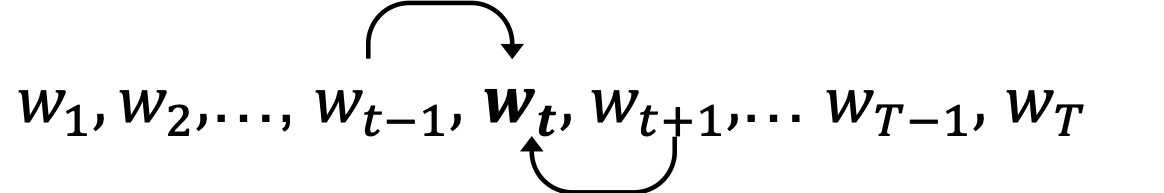
\includegraphics[width = 80mm]{image/cbow_w1w2wt-1wtwt+1.png}
  \caption{単語の列からターゲットとなる単語を推測する($m = 1$)}
  \label{fig:CBOWformula}
\end{figure}

\begin{figure}[H]
  \centering
  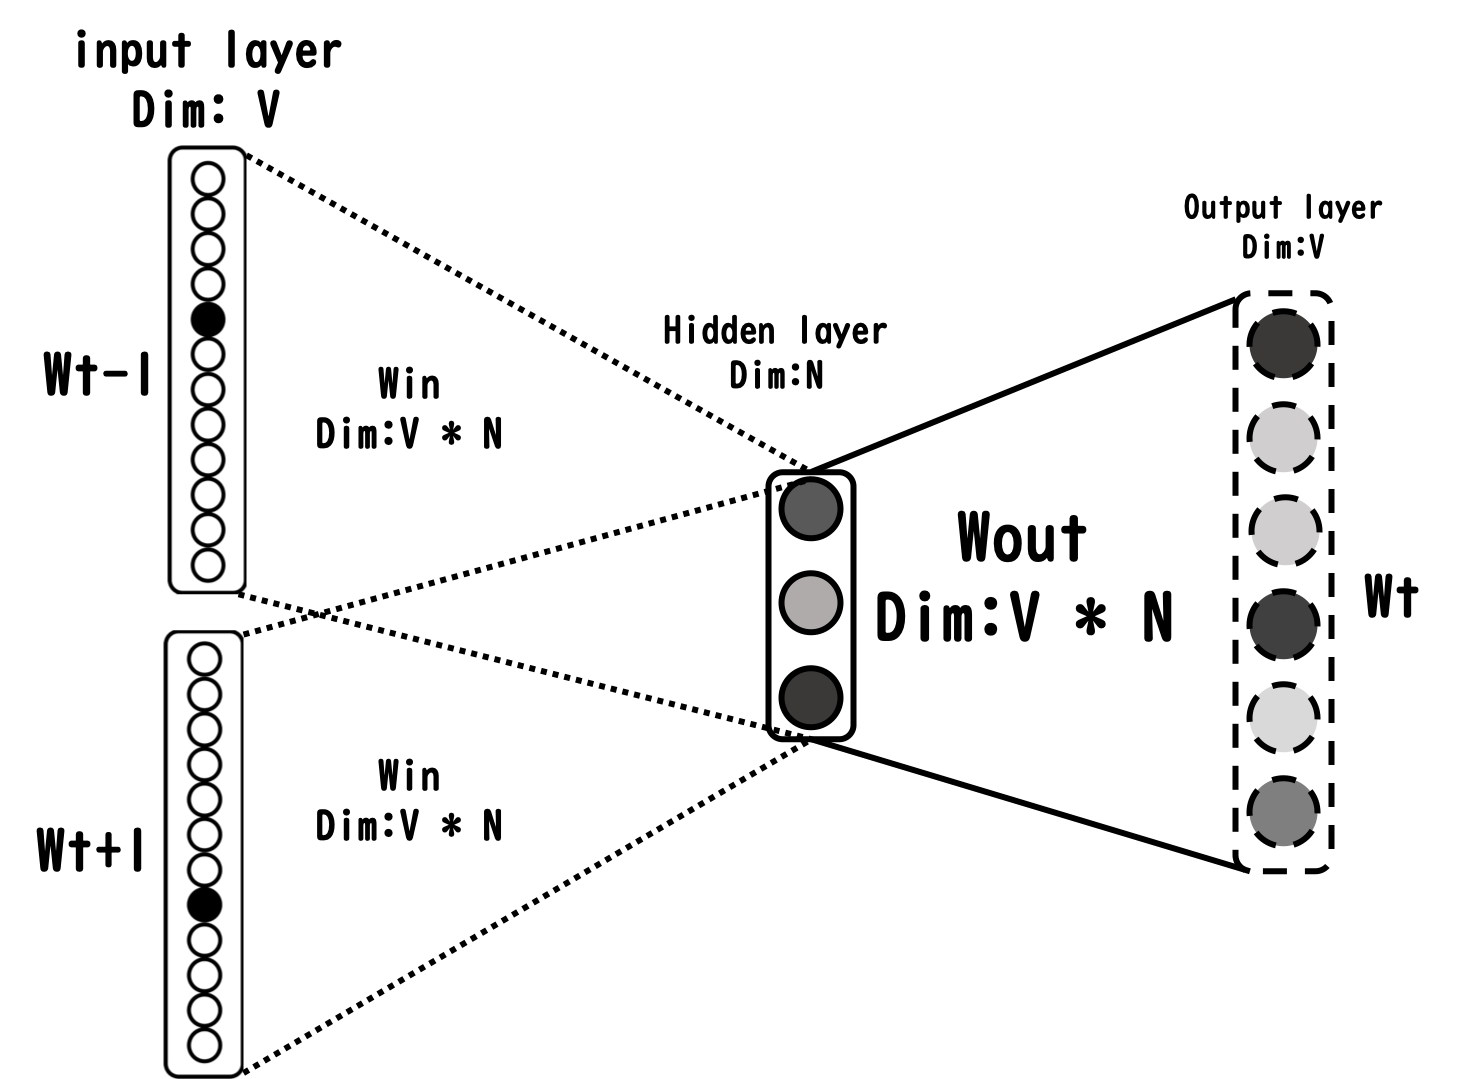
\includegraphics[width = 100mm]{image/CBOW_windowsize_1.png}
  \caption{CBOWのネットワーク構成モデル模式図($ m = 1$) }
  \label{fig:CBOWimage}
\end{figure}



\section{Skip Gram \label{sec:SkipGram}}
Skip Gramは文献\cite{SkipCBOW}で紹介されている\ref{sec:CBOW}章で述べたCBOWとは別の手法である.
CBOWとは逆に中心の単語$w_{t}$から前後$m$個の単語を推測するモデルである.
ネットワーク構成は図\ref{fig:SkipGramimage}のようになる.

\begin{figure}[H]
  \centering
  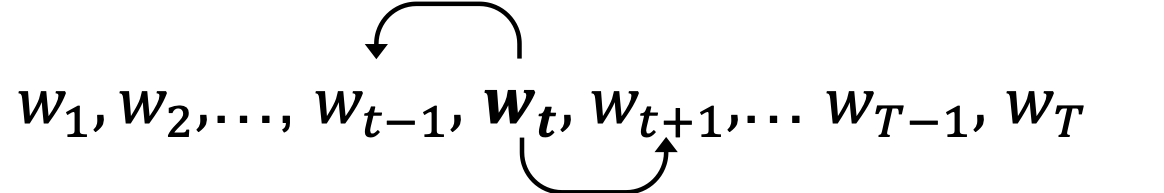
\includegraphics[width = 80mm]{image/skipgram_w1w2wt-1wtwt+1.png}
  \caption{単語の列からターゲットとなる単語を推測する($m = 1$)}
  \label{fig:Skipformula}
\end{figure}


\begin{figure}[H]
  \centering
  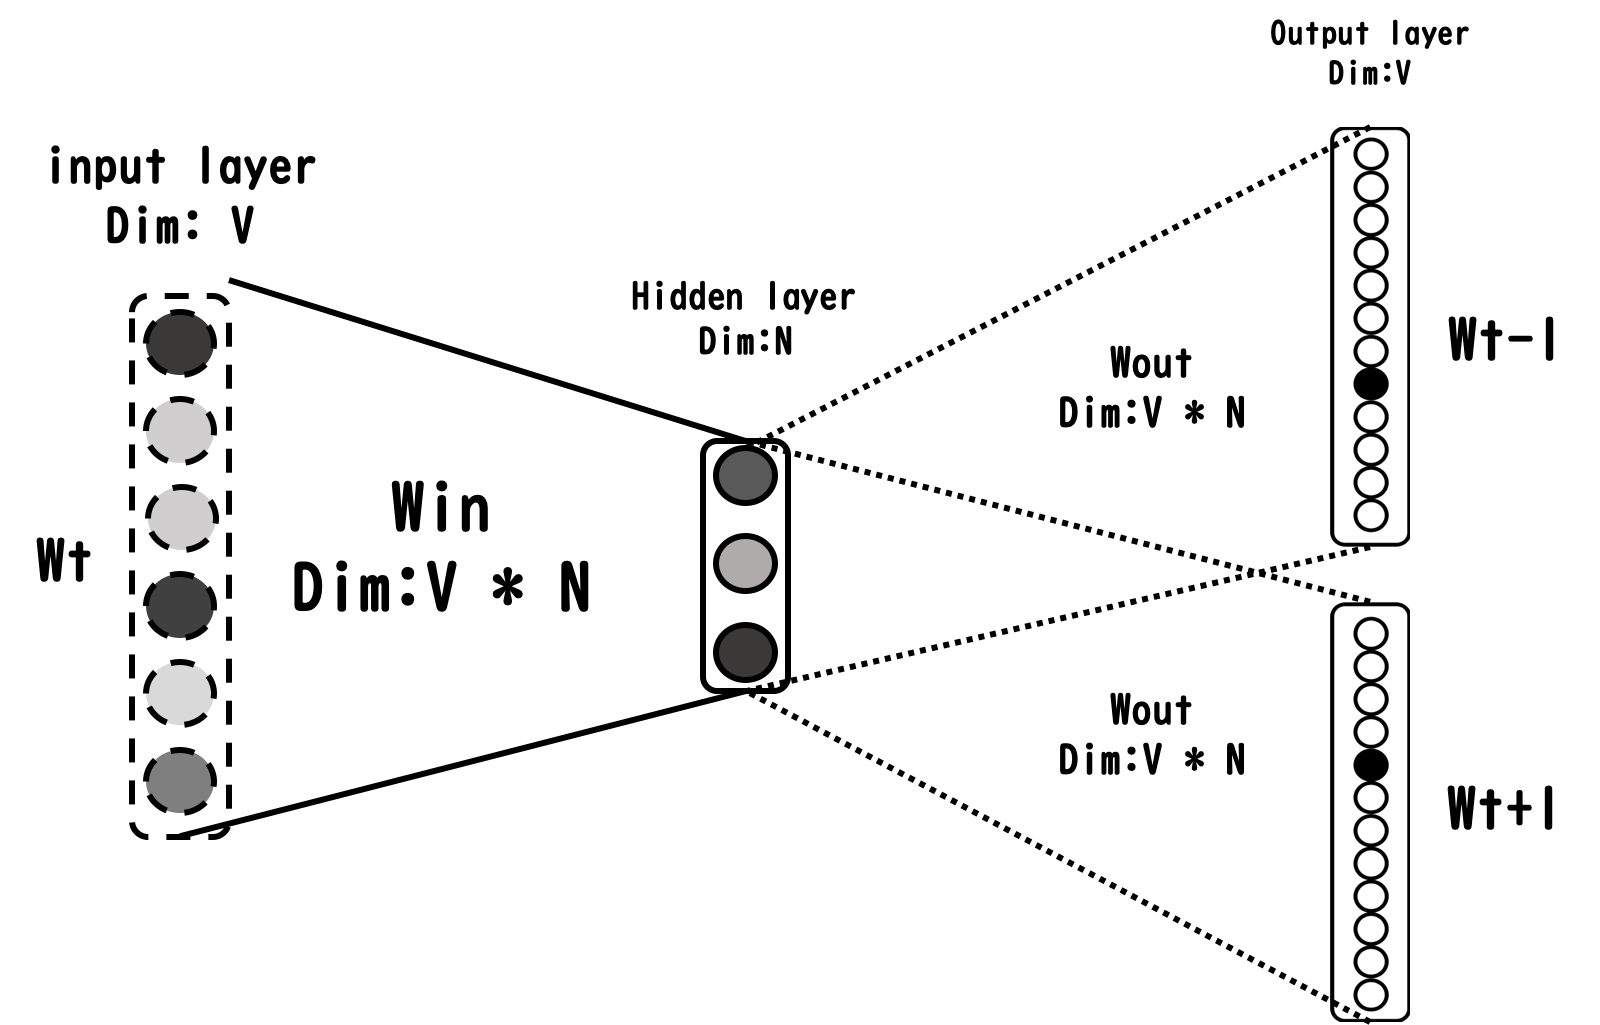
\includegraphics[width = 100mm]{image/SkipGram_windowsize_1.png}
  \caption{SkipGramのネットワーク構成モデル模式図($ m = 1$) }
  \label{fig:SkipGramimage}
\end{figure}



ある単語$w_{t}$が入力層に入力され,周辺単語の$w_{t-m},...,w_{t+m}$を推測する時,その全てが同時に起こる確率は式\ref{skip_probality}となる.

\begin{equation}
  \label{skip_probality}
  \begin{array}{c}
    P(w_{t-m},...,w_{t+m}|w_{t})
  \end{array}
\end{equation}

ここでSkipGramモデルは$w_{t-m},...,w_{t+m}$のそれぞれのあいだに関係性がないと仮定し,交差エントロピーを用いて損失関数(式\ref{skip_lossfunc})を定義する.

\begin{equation}
  \label{skip_lossfunc}
  \begin{split}
    -\log P(w_{t-m},...,w_{t+m}|w_{t} ) &= -\log \prod_{k = 1}^m P(w_{t-k}|w_{t}) \log P(w_{t+k}|w_{t})  \\
    &= - \sum_{k = 1}^m  ( \log P(w_{t-k} | w_{t}) + \log P(w_{t+k}|w_{t}) )
  \end{split}
\end{equation}

そして式\ref{skip_lossfunc}をコンテキスト$C$をコーパス全体に拡張すると式\ref{skip_loss}となり,この式を学習によって最小化していく.

\begin{equation}
  \label{skip_loss}
  \begin{split}
    - \sum_{C} \log P(w_{t-m},...,w_{t+m}|w_{t} ) &= \sum_{C} -\log \prod_{k = 1}^m P(w_{t-k}|w_{t}) P(w_{t+k}|w_{t})   \\
    &= - \sum_{C} \sum_{k = 1}^m \log P(w_{t-k} | w_{t}) + \log P(w_{t+k} | w_{t})
  \end{split}
\end{equation}


\chapter{LSTM(Long short-term memory)\label{ch:LSTM}}
順伝播ニューラルネットワークでは前の情報はつかわないため,文章や音声など,一つ前の情報に影響を受けるデータに対しては有用ではない.
そこで,ある時刻$t$の出力の際,過去の情報も扱う再帰ニューラルネットワーク(以降 RNN と省略)というものが発案された.

しかしながら通常のRNNの場合,時間が経つほどに前の情報は薄れていく勾配消失が起こることがあった.
これを解決しようとしたのが記憶情報ごとにメモリーの役割を果たすネットワークを分けたLong short-term memory(以降,LSTMと省略)というモデルである.

LSTMでは前の時刻$t-1$の$C_{t-1}$,$h_{t-1}$,現時刻の$x_{t}$を入力ベクトルとして受け取る.
$C_{t-1}$はLSTMで導入された時刻0から$t-1$ までの情報を記録しているベクトル,$h_{t-1}$は一時刻前の出力ベクトル,$x_{t}$は時刻$t$の入力ベクトルである.
それぞれのセルを計算するために4つのゲートを導入する.それぞれのゲートは入力セルの情報をどれくらい加味するかを重み付けするゲートである.
様々なバージョンがある中でもっとも基本的なネットワーク構成を模式図を図\ref{fig:LSTM_Simple}に示す.以下各ゲートに対して説明する.


\begin{figure}
  \centering
  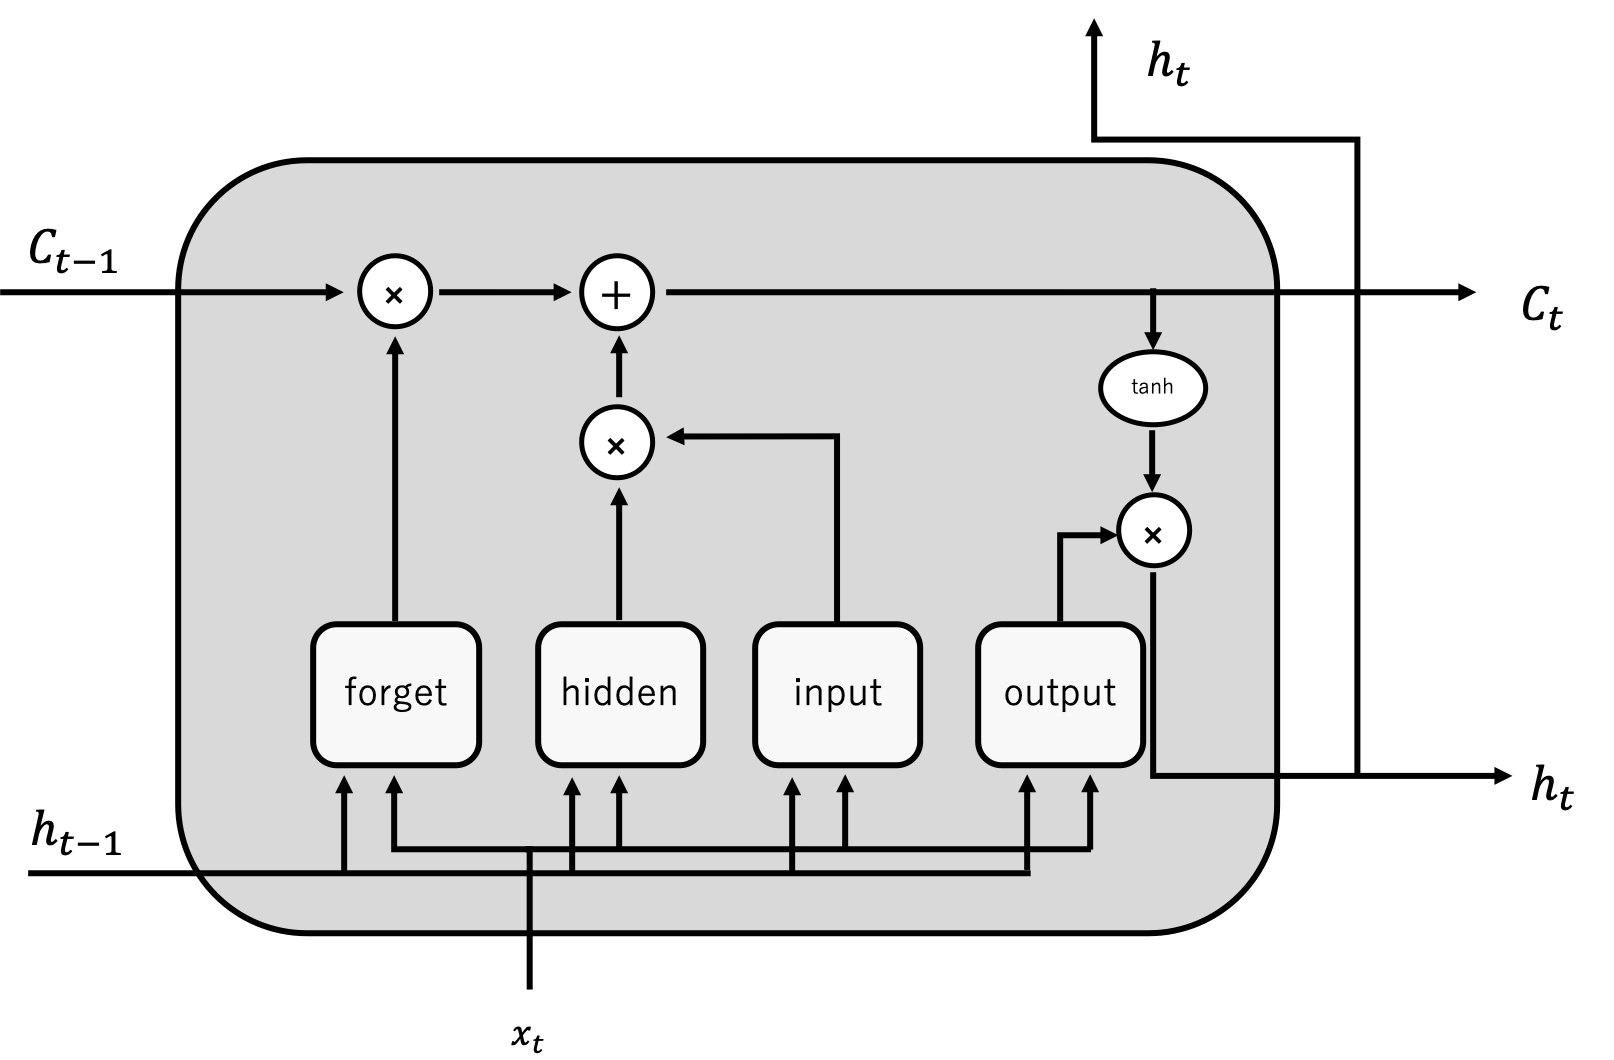
\includegraphics[width = 100mm]{image/lstm_simple_image.png}
  \caption{LSTMのネットワーク構成モデル模式図:図中のforget,hidden,input outputはそれぞれゲートが扱う情報を示している }
  \label{fig:LSTM_Simple}
\end{figure}

\section{forgetゲート\label{sec:forget}}
forgetゲートは過去の情報が詰まっている$C$セルをどの程度次の今の時刻に使うかを決める重みである.
その重みの計算には入力と一時刻前の隠れ層の出力が使われている(式\ref{eq:forget}).

\begin{equation}
  \label{eq:forget}
  \begin{split}
    f = sigmoid(x_{t}W_{x}^{(f)} + h_{t-1}W_{h}^{(f)} + b^{(f)})
  \end{split}
\end{equation}



\section{outputゲート\label{sec:output}}
ouputゲートでは次の時刻にどれくらい現在の情報を渡すかを決める重みである.
その重みの計算には入力と一時刻前の隠れ層の出力が使われている(式\ref{eq:output}).


\begin{equation}
  \label{eq:output}
  \begin{split}
    o = sigmoid(x_{t}W_{x}^{(o)} + h_{t-1}W_{h}^{(o)} + b^{(o)})
  \end{split}
\end{equation}

\section{hiddenゲート\label{sec:hidden}}

hiddenゲートではforgetゲートで差し引かれた記憶セル$C$に新たな情報を加えるゲートである.
その情報は入力と一時刻前の隠れ層の出力を用いて算出する(式\ref{eq:hidden}).


\begin{equation}
  \label{eq:hidden}
  \begin{split}
    \bar{h} = \tanh(x_{t}W_{x}^{(h)} + h_{t-1}W_{h}^{(h)} + b^{(h)})
  \end{split}
\end{equation}

\section{inputゲート\label{sec:input}}

inputゲートではhiddenゲートで追加しようとした新たな記憶をどのくらい加算するかを決める重みを求めるゲートである.
その重みの計算には入力と一時刻前の隠れ層の出力が使われている(式\ref{eq:input}).


\begin{equation}
  \label{eq:input}
  \begin{split}
    i = sigmoid(x_{t}W_{x}^{(i)} + h_{t-1}W_{h}^{(i)} + b^{(i)})
  \end{split}
\end{equation}


\section{LSTMのまとめ}
\ref{eq:forget}節,\ref{sec:output}節,\ref{sec:input}節,\ref{eq:hidden}節で紹介したものをまとめると式\ref{eq:all}のようになる.


\begin{equation}
  \label{eq:all}
  \begin{split}
    f &= sigmoid(x_{t}W_{x}^{(f)} + h_{t-1}W_{h}^{(f)} + b^{(f)}) \\
    o &= sigmoid(x_{t}W_{x}^{(o)} + h_{t-1}W_{h}^{(o)} + b^{(o)}) \\
    \bar{h} &= \tanh(x_{t}W_{x}^{(h)} + h_{t-1}W_{h}^{(h)} + b^{(h)}) \\
    i &= sigmoid(x_{t}W_{x}^{(i)} + h_{t-1}W_{h}^{(i)} + b^{(i)})
  \end{split}
\end{equation}

\begin{equation}
  \label{eq:all2}
  \begin{split}
    C_{t} &= f \odot c_{t-1} + g \odot i
  \end{split}
\end{equation}

\begin{equation}
  \label{eq:all3}
  \begin{split}
    h_{t} &= o \odot \tanh(C_{t})
  \end{split}
\end{equation}

LSTMモデルを3時刻分展開したものを図\ref{fig:LSTM_3timeconcat}に示す.

\begin{center}
  \begin{figure}[H]
    \centering
    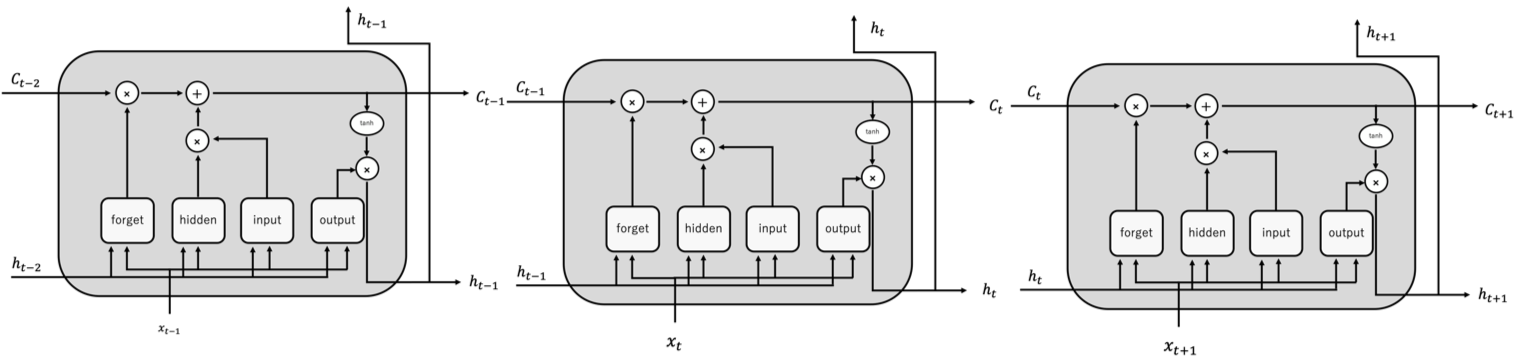
\includegraphics[width=\linewidth]{image/LSTM_concat.png}
    \caption{LSTMの3時刻展開:記憶を守る機構によりより高い濃度で次の時刻に情報を渡すことができる}
    \label{fig:LSTM_3timeconcat}
  \end{figure}
\end{center}






\chapter{系列変換\label{ch:Seq2Seq}}

系列変換とは再帰ニューラルネットワークを用いて時系列データを時系列データに変換することをさす.
モデルの構成図の例を図\ref{fig:seq2seq_3time}にしめす.

\begin{center}
  \begin{figure}[tbh]
    \centering
    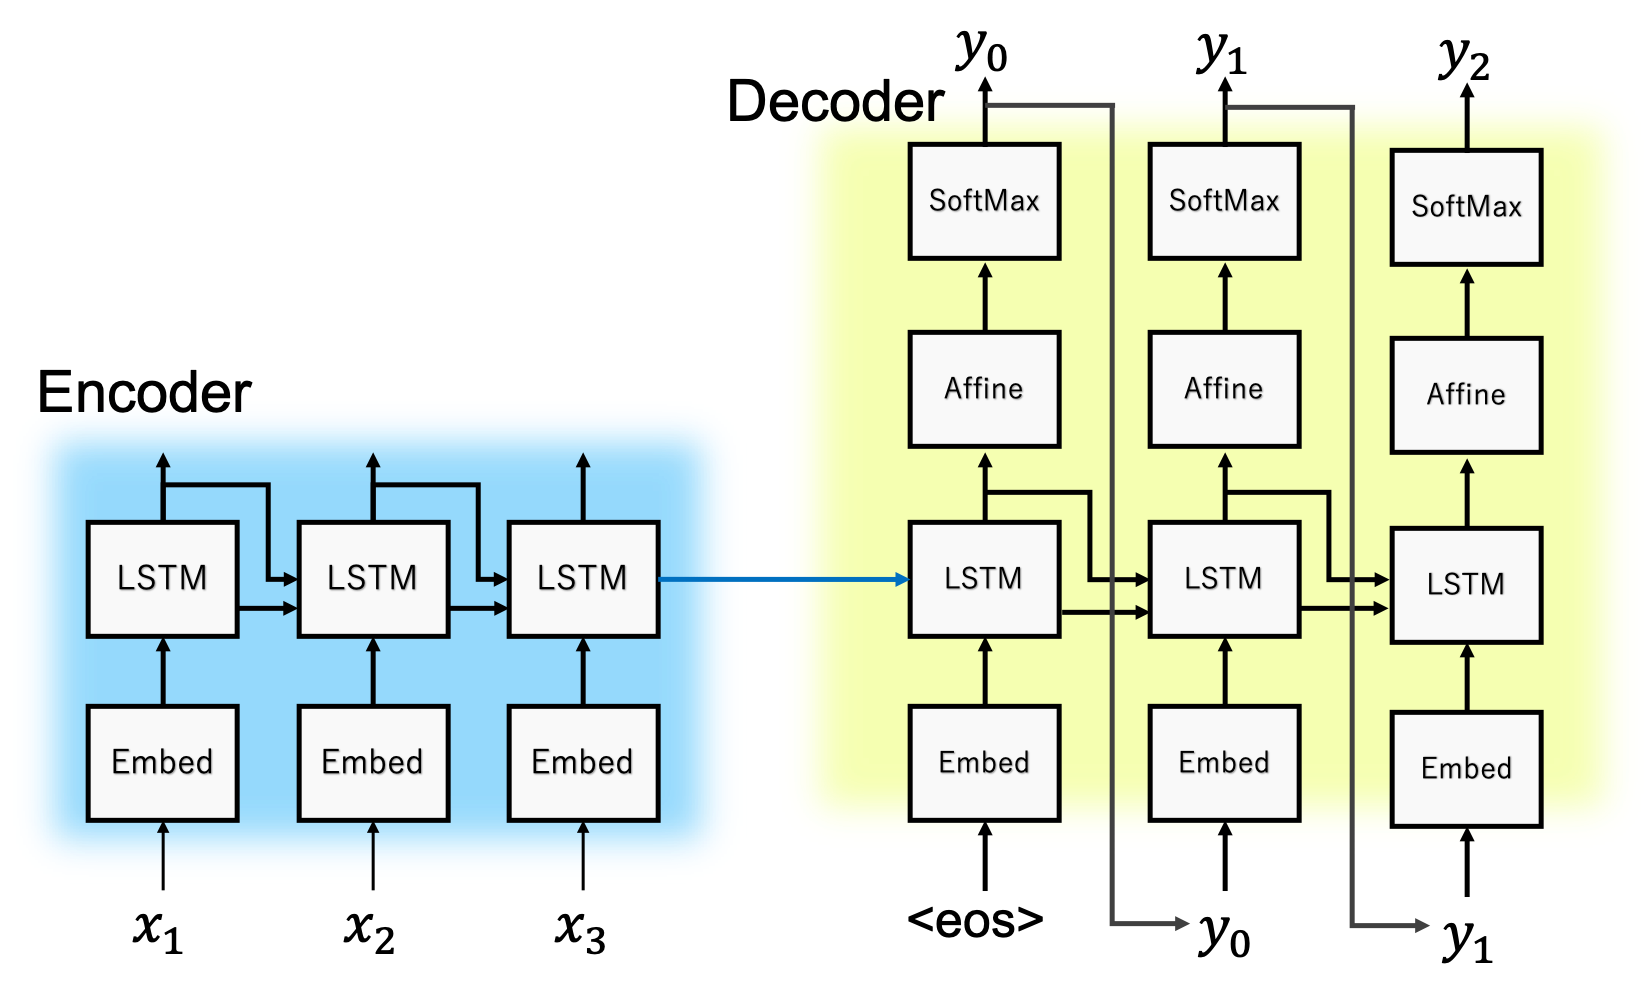
\includegraphics[width=\linewidth]{image/seq2seq_image.png}
    \caption{LSTMを用いた基本的な系列変換モデルの3時刻展開 }
    \label{fig:seq2seq_3time}
  \end{figure}
\end{center}

大きく分けてEncoderとDecoderに分かれる.Encoder側は入力を受け取りEmbedding層で入力系列$x_{i}$を埋め込み行列に変換し,
LSTMに入力として渡す.EncoderではLSTMが時系列データを記憶するメモリーのように振る舞い次の時刻へ情報を渡していく,
時刻$t$の時のLSTMの隠れ層の出力$h_{t}$にはLSTMが渡してきた$1 \sim t$までの情報が溜め込まれており,入力系列を変換するために必要な情報が
エンコードされて任意の固定長ベクトルに溜め込まれる.
この固定長ベクトルDecoder側の最初のLSTMの前の時刻の$h$として入力され,区切り文字$<$EOS$>$を入力として受け取り,
Encoder側と同じように埋め込み行列に変換しLSTMで再帰的に学習,そしてAffine層で入力ベクトルの大きさと同サイズに圧縮し,
SoftMax層(式\ref{eq:softmax})でベクトルの値を確率に変換する.

\begin{equation}
  \label{eq:softmax}
  \begin{split}
    softmax(x)_{i} = \frac{ e^{x_{i}} }{ \sum_{i} e^{x_{i}} }
  \end{split}
\end{equation}

区切り文字$<$EOS$>$によって出力された$y_{0}$を次の時刻の入力とし,$2$時刻目として$y_{1}$を出力し再び区切り文字を出力するまで繰り返す.
この技術を応用して機械翻訳など時系列データを扱う.

\if0
\chapter{Attention\label{ch:attention} }
章\ref{ch:Seq2Seq}で導入した系列変換モデルだが,問題点があり,図\ref{fig:seq2seq_3time}で示したように,系列を固定長のベクトルに情報を溜め込むのだが,系列が長くても短くても固定長のベクトルになるため長い系列だと容量不足になる問題があった.
そのことを解決する手法の一つとしてAttentionを導入する.
Encoderの出力は時刻$t$の入力系列をベクトルに変換したものなので時刻$t$の出力がもっとも時刻$t$の状態を反映した物であるという仮定のもと,
AttentionではDecoder側で出力系列を生成するとき,出力と対応するEncoderの出力ベクトルに注意して生成するようにする.
これをAttention(注意機構)という.
章\ref{ch:Seq2Seq}の図\ref{fig:seq2seq_3time}にAttentionを加えたネットワークを図\ref{fig:Attention_3time}に示す.




\begin{center}
  \begin{figure}[h]
    \centering
    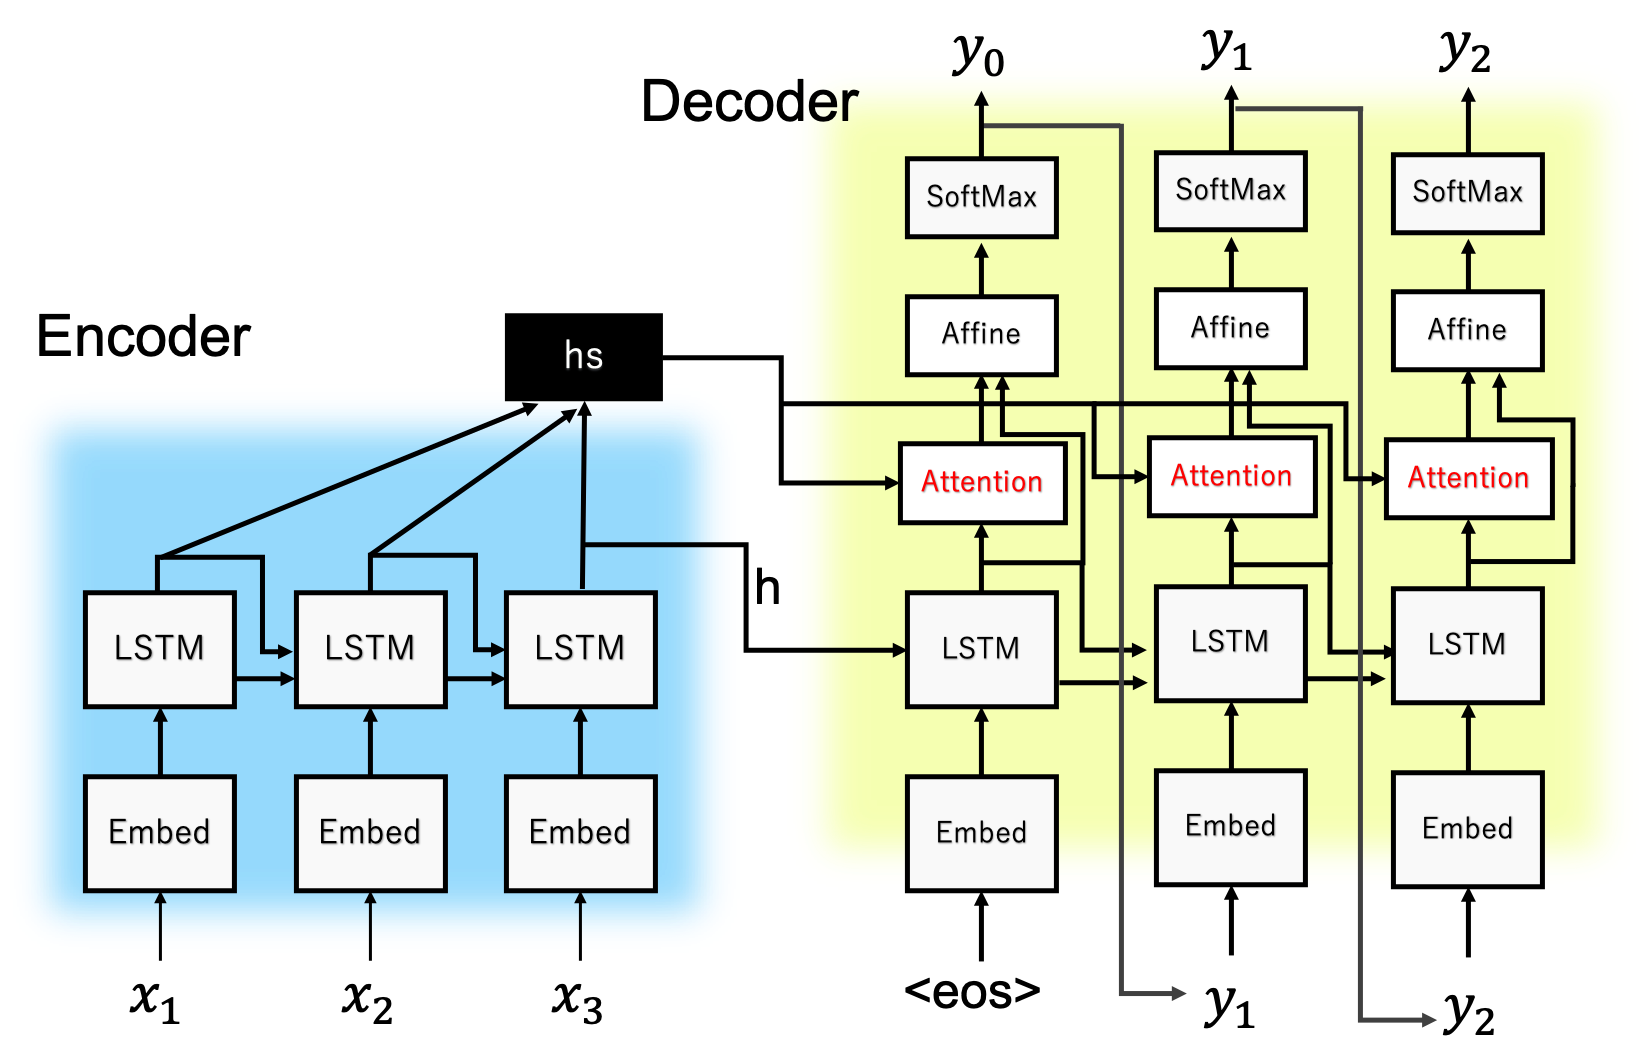
\includegraphics[width=\linewidth]{image/attention_image.png}
    \caption{LSTMを用いた基本的な系列変換モデルの3時刻展開にAttenitonを追加したネットワーク }
    \label{fig:Attention_3time}
  \end{figure}
\end{center}



Encoder側では各時刻の出力を$hs$として溜め込んでいく.
Decoder側ではLSTNを抜けた隠れ層の出力ベクトルを$h^{decoder}$とすると図\ref{fig:Attention_3time}で行うAttentionの計算の概要を
図\ref{fig:Attention_layer}に示す.
Attention Weightはhsと$h^{decoder}$のベクトルの類似度を計算する.その過程を式\ref{eq:AttentionWeight}に示す.

\begin{equation}
  \label{eq:AttentionWeight}
  \begin{split}
    s = hs \odot h^{decoder}  \\
    a = softmax(s)
  \end{split}
\end{equation}

二つのベクトルを内積をとることにより類似度に変換し,その後SoftMax(式\ref{eq:softmax})で変換する.この類似度のベクトルをScoreともいう.

またWeight SumではこのScoreを元にhsのどこに注意を置くのかを算出する.その過程を式\ref{eq:WeightSum}に示す.
よってContextVecterはEncoderの入力系列の重要なところを注視したベクトルが作られ,これをDecoderのLSTMの出力値とconcatし読み込むことでその性能を格段に向上させることに成功している.(文献\cite{attention})


\begin{equation}
  \label{eq:WeightSum}
  \begin{split}
    c = \sum_{i} hs_{i} a_{i}
  \end{split}
\end{equation}

\begin{center}
  \begin{figure}[ht]
    \centering
    \includegraphics[width=0.5\linewidth]{image/attention_layer.png}
    \caption{Attention内部で行う計算  Attention Weightはベクトルの類似度を計算し,Weight Sumは類似度からhsをどれくらい重要視するかを示すContextVecterを算出する}
    \label{fig:Attention_layer}
  \end{figure}
\end{center}
\fi


\chapter{Exericises Vecter Representation\label{ch:method}}
\if0
\point{
自分の提案する解決方法を説明する.
\begin{itemize}
  \item 章題は適切なものに変えること.章をわけてもよい.
  \item 必ず具体例を用いること.
  \item 最初に問題を解く上で最も難しい点とそれを解決するアイデアを示す.
  \item 詳細については,全体の流れを示した後,各ステップについて説明する.
  \item 検討時に行った予備評価の結果があれば示す.
\end{itemize}
}
\fi

\section{システム全体の流れ}

数式の特徴を取り出し$S$次元のベクトルに変換し,その分布から類題選出を行うシステムの
概要を図\ref{fig:EVS_Simple}に示す,
ExericisesEncoderは数式を数式をベクトル 表現に変換し蓄積する.
その変換結果のベクトルと間違えた問題も同様の手段でベクトル化し蓄積した式のベクトル表現との類似度を算出し,
その類似度が高い式を類題として出力する.

\begin{center}
  \begin{figure}[H]
    \centering
    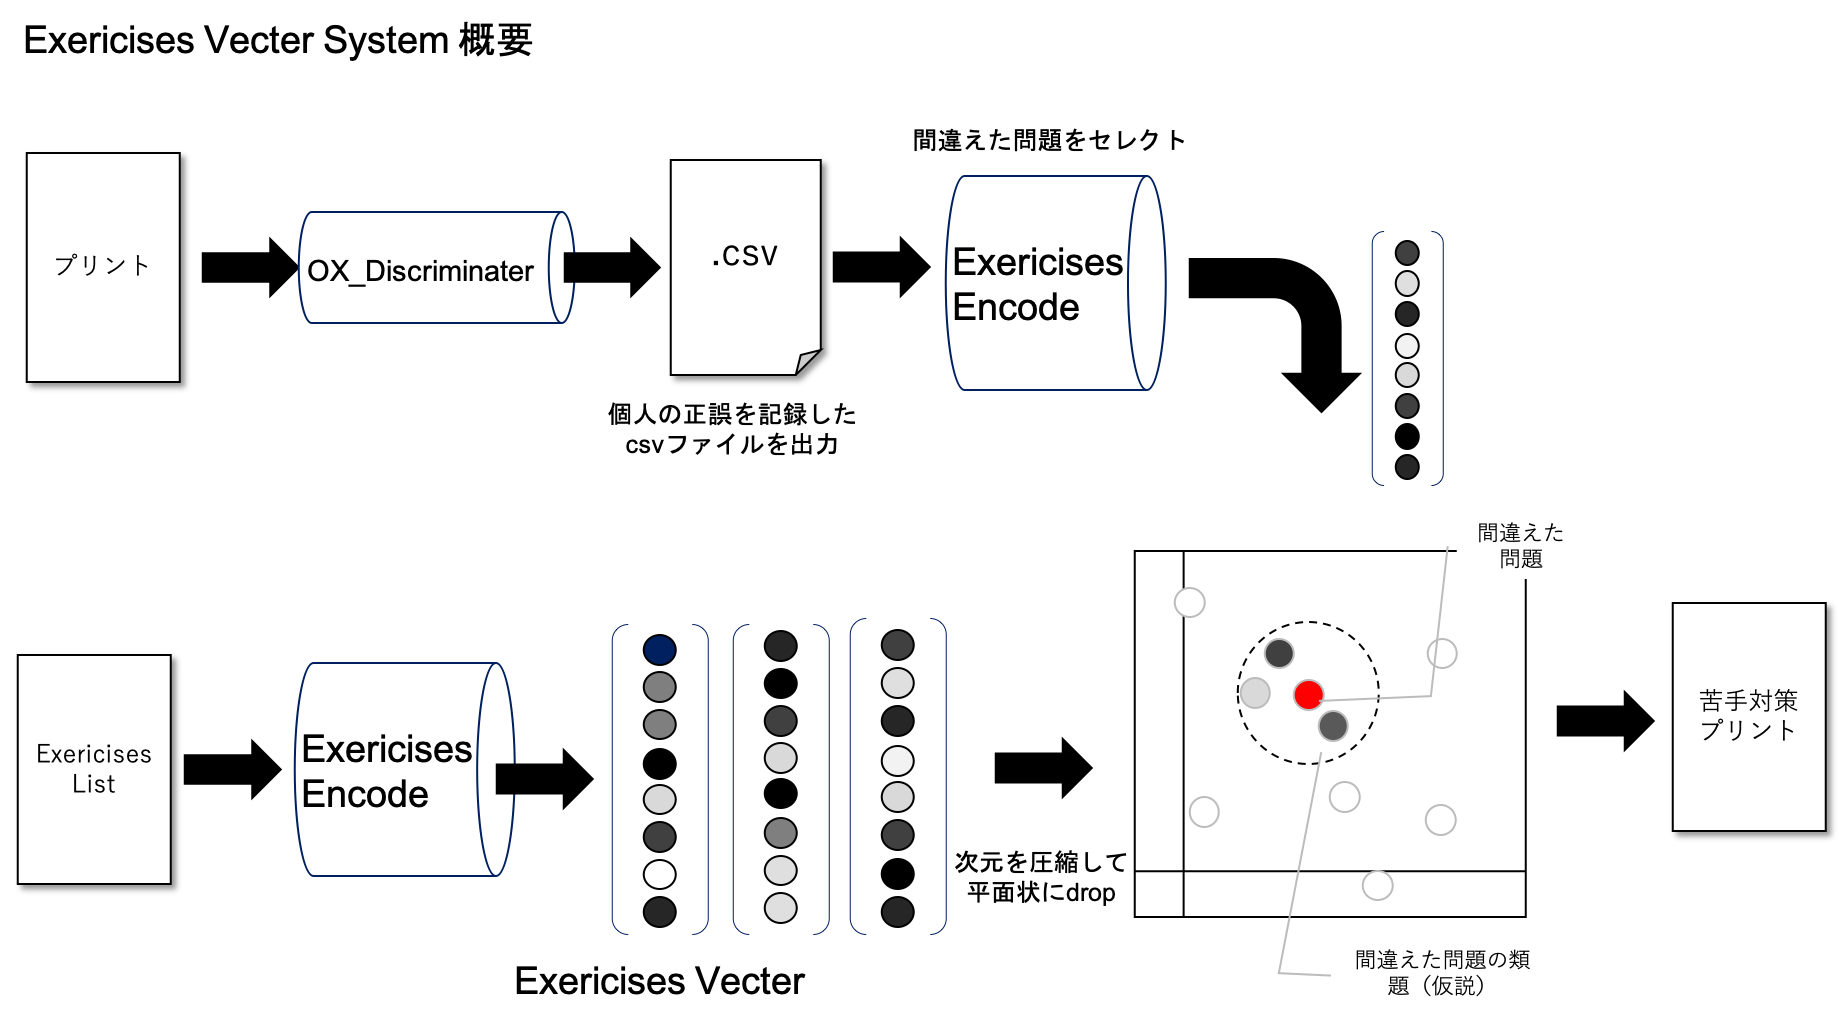
\includegraphics[width=\linewidth]{image/EVS_Simpie.png}
    \caption{ExericisesEncoder 模式図}
    \label{fig:EVS_Simple}
  \end{figure}
\end{center}

\section{計算式の特徴量抽出}
\subsection{概要}
数式を分布化する際,そのベクトルの中に数式の特徴を入れ込んだベクトルを生成する手法が確立していない.そこで本論文では数式の各文字,記号を単語のようにみなし,onehotベクトルを作成し,それを埋め込み層で特徴を踏まえたベクトルに変換したのち,系列変換モデルで読み込むことで数式の特徴を掴んだベクトルを生成できないかと考えた.

この考えを実現するために数式は我々が目にする$2x+3=5$, $\frac{3x-1}{2}+4=\frac{2}{5}$ではなく,テキスト化かつその特徴を強く受けた形に変換する必要がある.
そこで本論文では数式をある一定のルールの中でテキスト化されている{\TeX}形式の数式を用いる.
上記の計算式なら\verb#2x+3=5#,\verb#\frac{3x-1}{2}+4=\frac{2}{5}#とし,このテキストデータを用いて文字単位の埋め込んだベクトルを作成する.
この式を数字,文字,小数点,符号,丸括弧,波括弧でわけそれぞれonehot表記でベクトル化する.

実験で用いた分散表現獲得手法は以下の2手法である.
\begin{itemize}
  \item CBOW
  \item SkipGram
\end{itemize}


\subsection{文字分布の予備実験結果}
予備実験として埋め込み層に利用するCBOW,SkipGramで文字の特徴が得られているかを確認した.
学習データとして350種類の一次方程式の問題を用いた.
その一部を以下に示す.


\begin{multicols}{2}
  \begin{quote}
    \verbatimtabinput[3]{collection2.txt}
  \end{quote}
\end{multicols}

以降,\verb#\frac#を$f$と表記し,
上記の式を$f,\{,\},(,),x,=,+,-,.,0,1,2,3,4,5,6,7,8,9,$ $<$EOS$>$,$<$UNK$>$を語彙としてonehotベクトルに変換した.
埋め込みベクトルの次元数は200次元とした.
結果を図\ref{fig:89x2cbow_pac}$\sim$図\ref{fig:22x2skip_tsne}に示す

\begin{center}
  \begin{figure}[H]
    \centering
    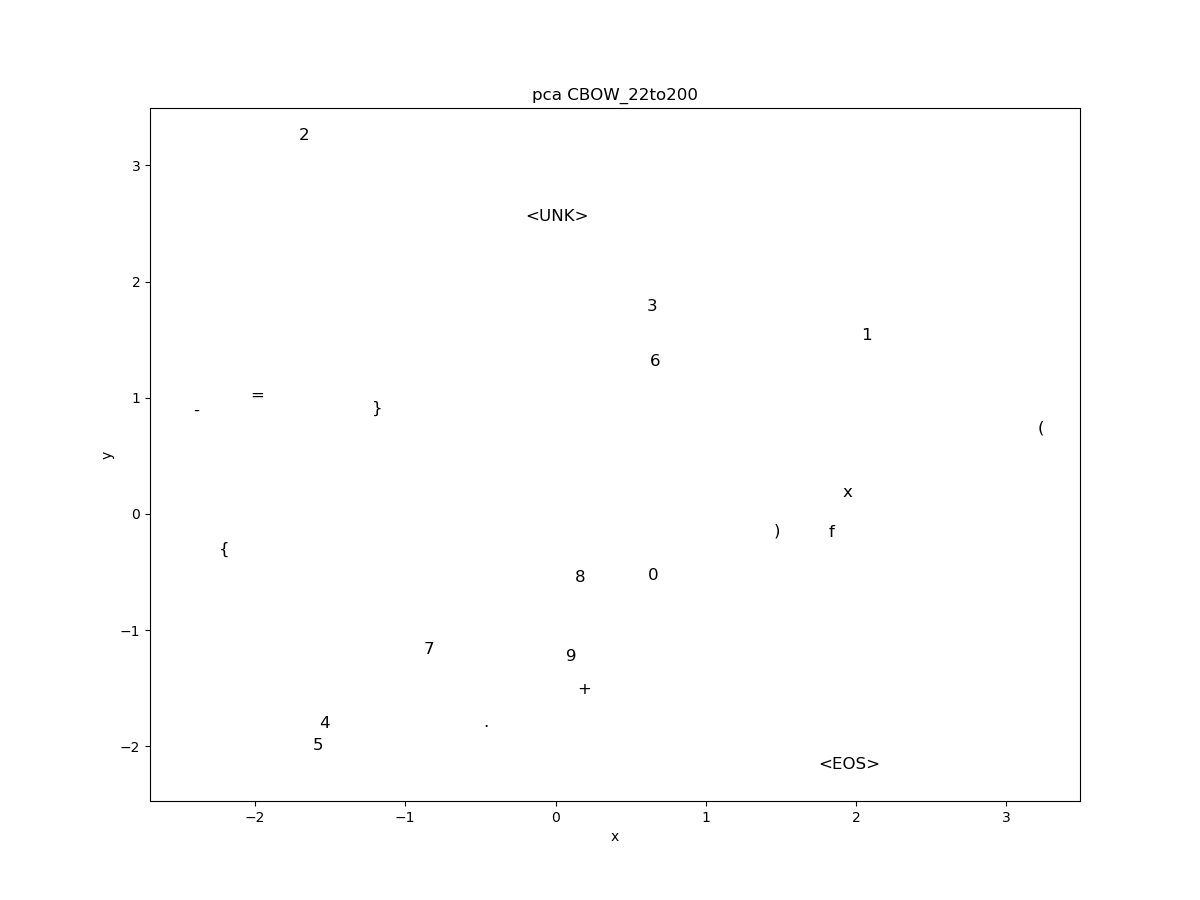
\includegraphics[width=0.8\linewidth]{image/CBOW_pca_out22_200.png}
    \caption{CBOWにて22次元を200次元に分散表現を変換したのちPCAで再構成しグラフ化した結果}
    \label{fig:89x2cbow_pac}
  \end{figure}
\end{center}


\begin{center}
  \begin{figure}[H]
    \centering
    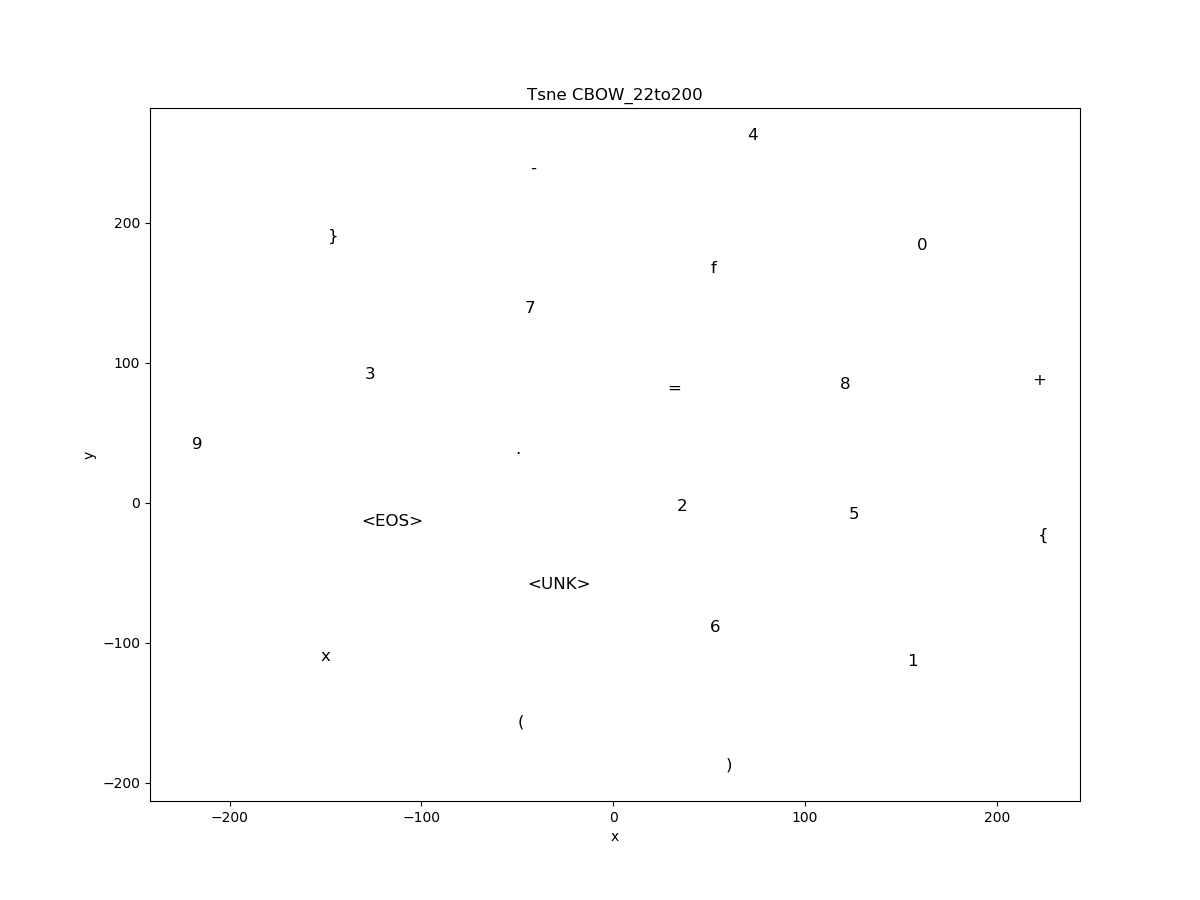
\includegraphics[width=0.8\linewidth]{image/CBOW_tsne_out22_200.png}
    \caption{CBOW 22次元を200次元に分散表現を変換したのちt-SNEで再構成しグラフ化した結果}
    \label{fig:89x2cbow_tsne}
  \end{figure}
\end{center}


\begin{center}
  \begin{figure}[H]
    \centering
    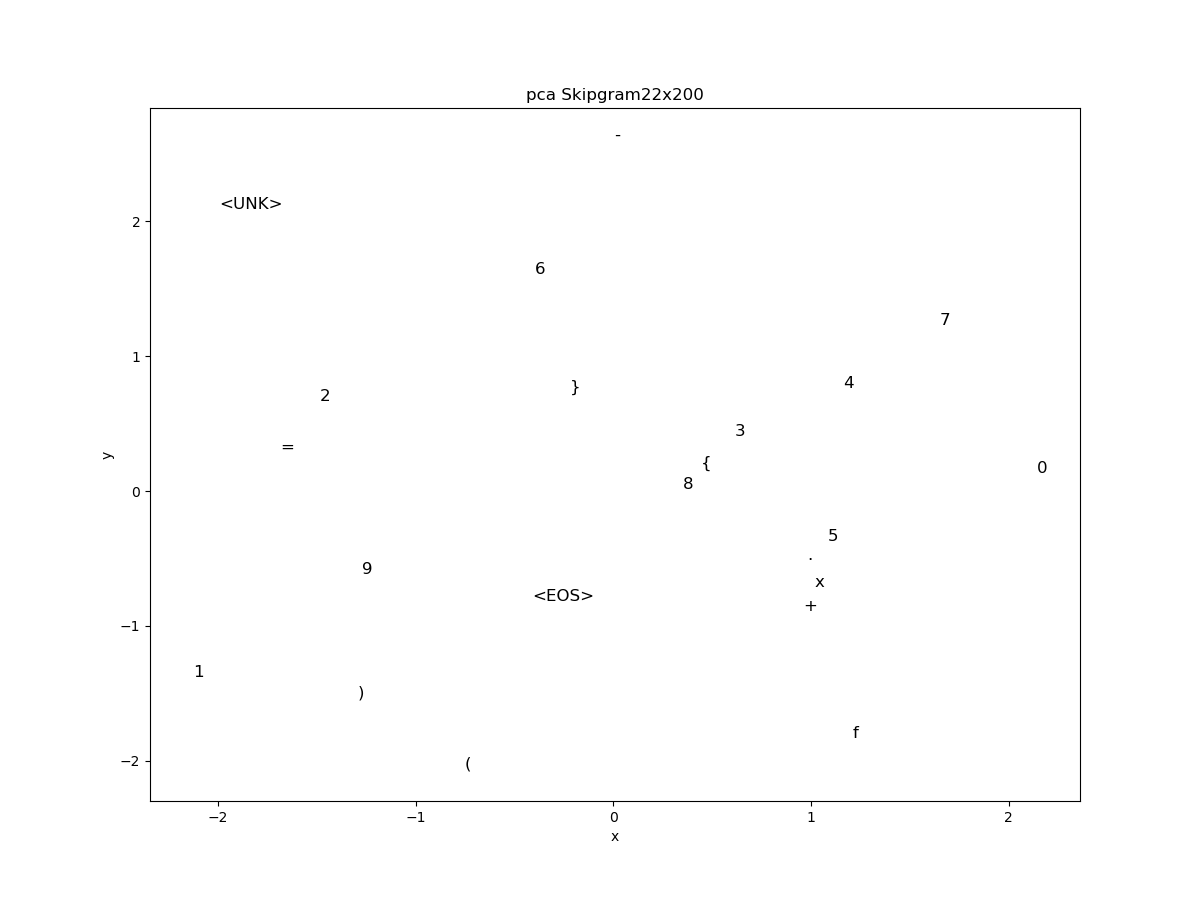
\includegraphics[width=0.8\linewidth]{image/pca_skipgram.png}
    \caption{SkipGramにて22次元を200次元に分散表現を変換したのちPCAで再構成しグラフ化した結果}
    \label{fig:22x2_skippca}
  \end{figure}
\end{center}


\begin{center}
  \begin{figure}[H]
    \centering
    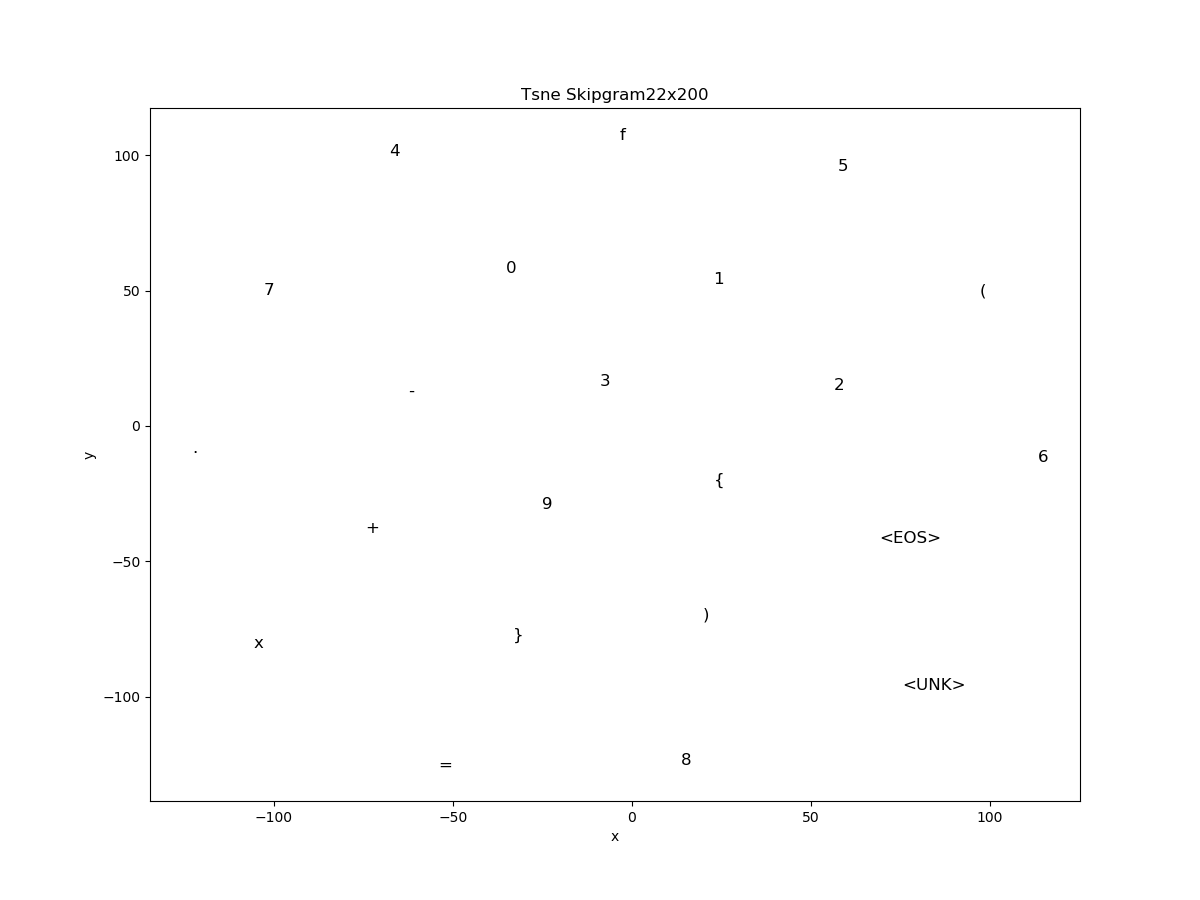
\includegraphics[width=0.8\linewidth]{image/tsne_skipgram.png}
    \caption{SkipGramにて 22次元を200次元に分散表現を変換したのちt-SNEで再構成しグラフ化した結果}
    \label{fig:22x2skip_tsne}
  \end{figure}
\end{center}

図\ref{fig:89x2cbow_pac}や図\ref{fig:89x2cbow_tsne}を見るとそれぞれの文字に関係はないように見える.
実際にベクトルの類似度のランキングは以下のようになった.
inputと書かれている横の文字が入力文字でその下に類似度の高い順に5つ並んでいる.
例えばfを入力した時では最も類似度が高いのが同じ文字のfであり,その下に1,(,0,9と続く.
\begin{multicols}{2}
  \begin{quote}
    \verbatimtabinput[3]{cbow_similer.txt}
  \end{quote}
\end{multicols}



これを見てもベクトル間に関係が現れていないように見える.文献\cite{seq2seq}のようにベクトル間の演算はできないが,
丸括弧$( , )$と波括弧$\{ , \}$のベクトル間距離を測ると
\[
( と ) の距離 27.04968437532474
\]
\[
\{ と \} の距離 27.04968437532474
\]
このように完全に一致した.このことからword2vecを数式に用いた場合, 数字自体の演算はできないが数式の形状は取り出せる事がわかった.

なお,ベクトル間の距離を式\ref{eq:l},類似度を式\ref{eq:inner}を用いて求めた.

\begin{equation}
  \label{eq:l}
  \begin{split}
    |\vec{a}-\vec{b}| =  \sqrt{|\vec{a}|^2 + |\vec{b}|^2 - 2  \vec{a} \cdot \vec{b}}
  \end{split}
\end{equation}

\begin{equation}
  \label{eq:inner}
  \begin{split}
    \cos \theta = \frac{\vec{a} \cdot \vec{b}}{|\vec{a}| |\vec{b}|}
  \end{split}
\end{equation}

\section{系列変換モデルの検討}
本論文では系列変換の過程で用いるEncoderからDecoderに渡す最終出力$h$を式ベクトルとしてみなす.
よって$h$の精度を高めていくモデルが必要となる.
\begin{itemize}
  \item 通常のLSTMで行う系列変換を多層に積み上げるモデル(図\ref{fig:seq2seq})
  \item 通常Decoderが側で利用されるSkipConnectionをEncoderで採用したSkipConnectionモデル(図\ref{fig:SkipSeq2seq})
  \item 前時刻の情報も用いるBi-Directional(図\ref{fig:bi-directionl Seq2seq}).

\end{itemize}
この三つを用いて実験を行った.

今回,この実験ではEncoder側がより精度の高いベクトルを生成してもらうことが目的なのでDecoder側は通常のLSTMを一層で行う系列変換で確認を行うこととした.

\begin{center}
  \begin{figure}[H]
    \centering
    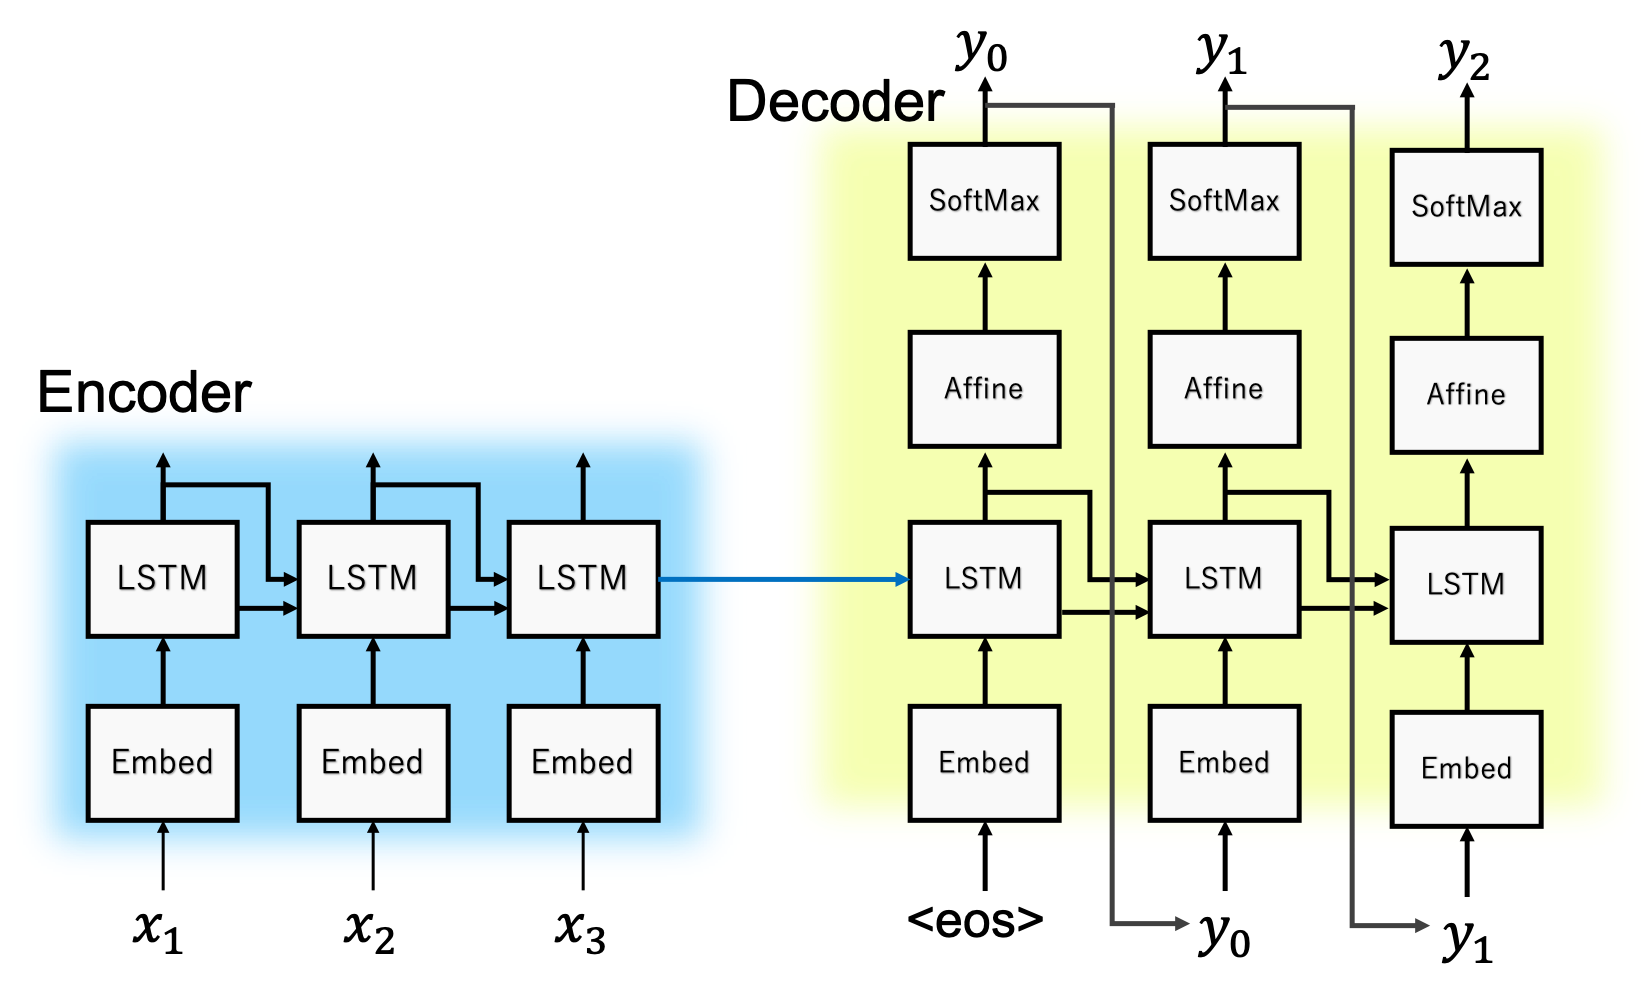
\includegraphics[width=0.9\linewidth]{image/seq2seq_image.png}
    \caption{基本モデル}
    \label{fig:seq2seq}
  \end{figure}
\end{center}

\begin{center}
  \begin{figure}[H]
    \centering
    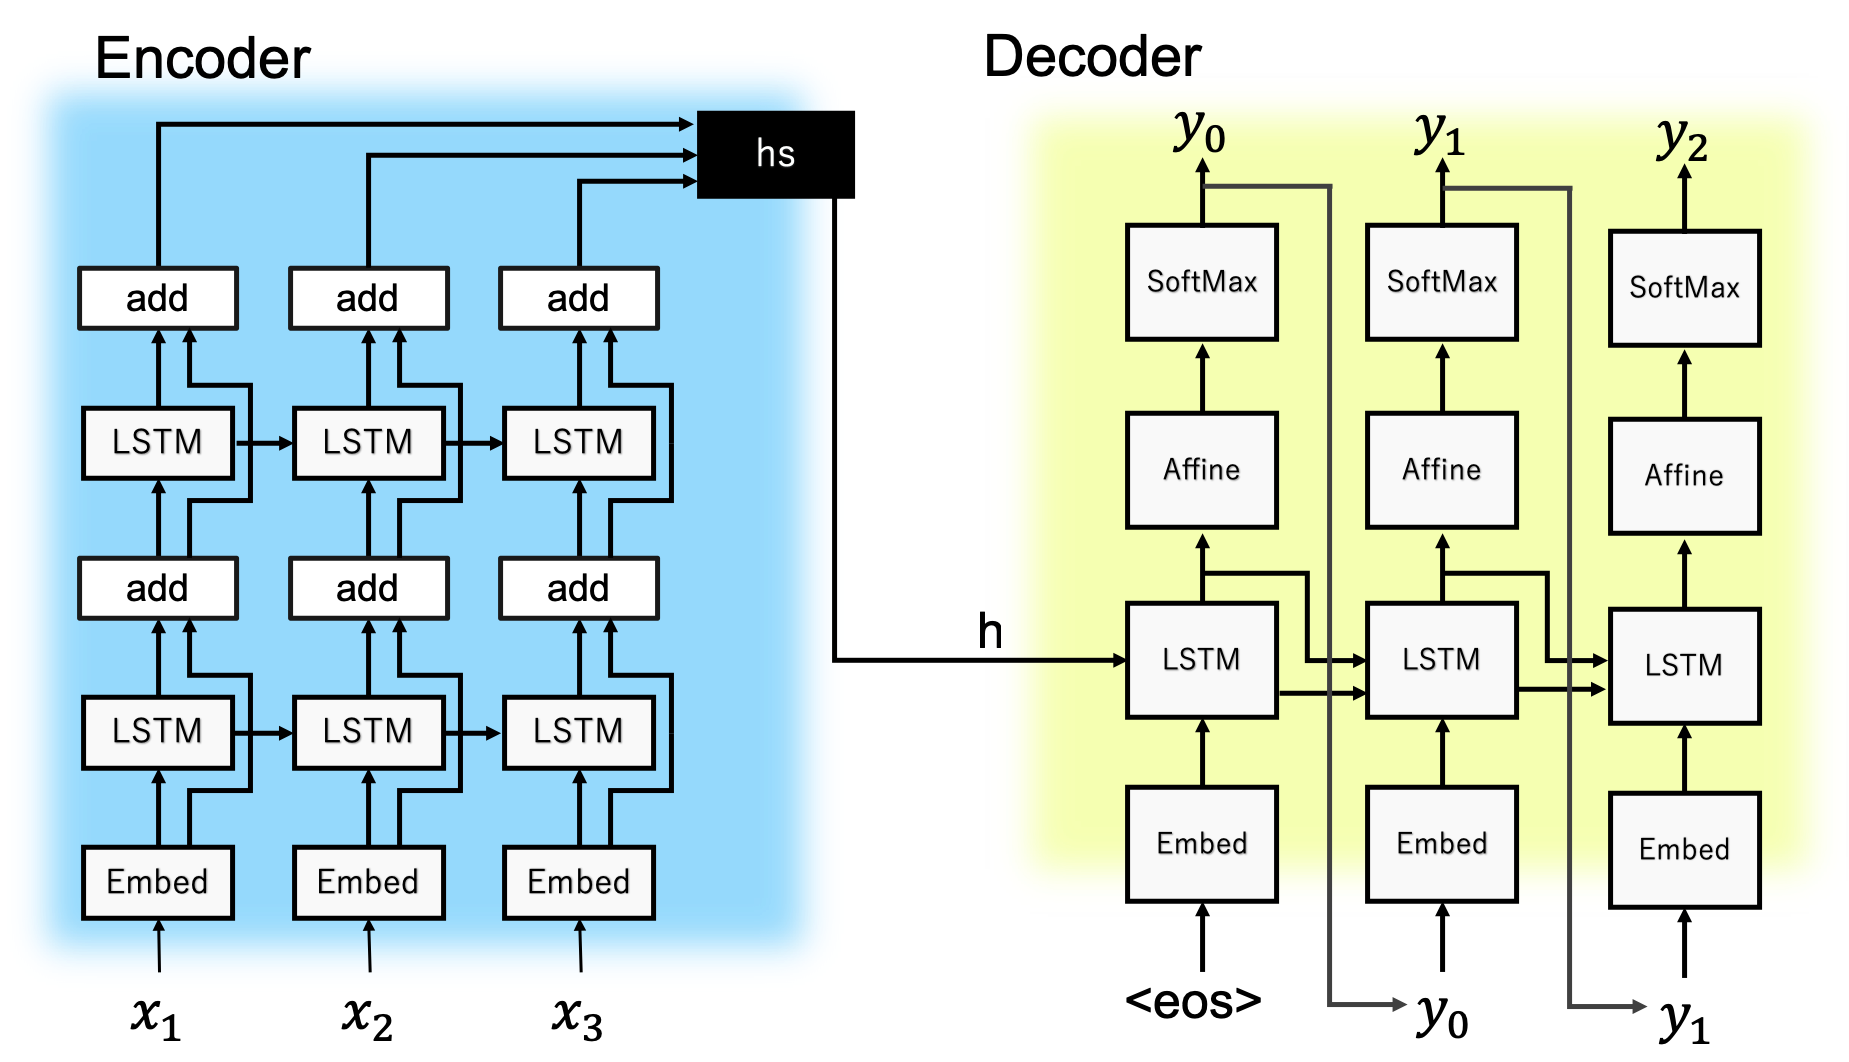
\includegraphics[width=0.9\linewidth]{image/Skipconnect.png}
    \caption{SkipConnectionモデル}
    \label{fig:SkipSeq2seq}
  \end{figure}
\end{center}

\begin{center}
  \begin{figure}[H]
    \centering
    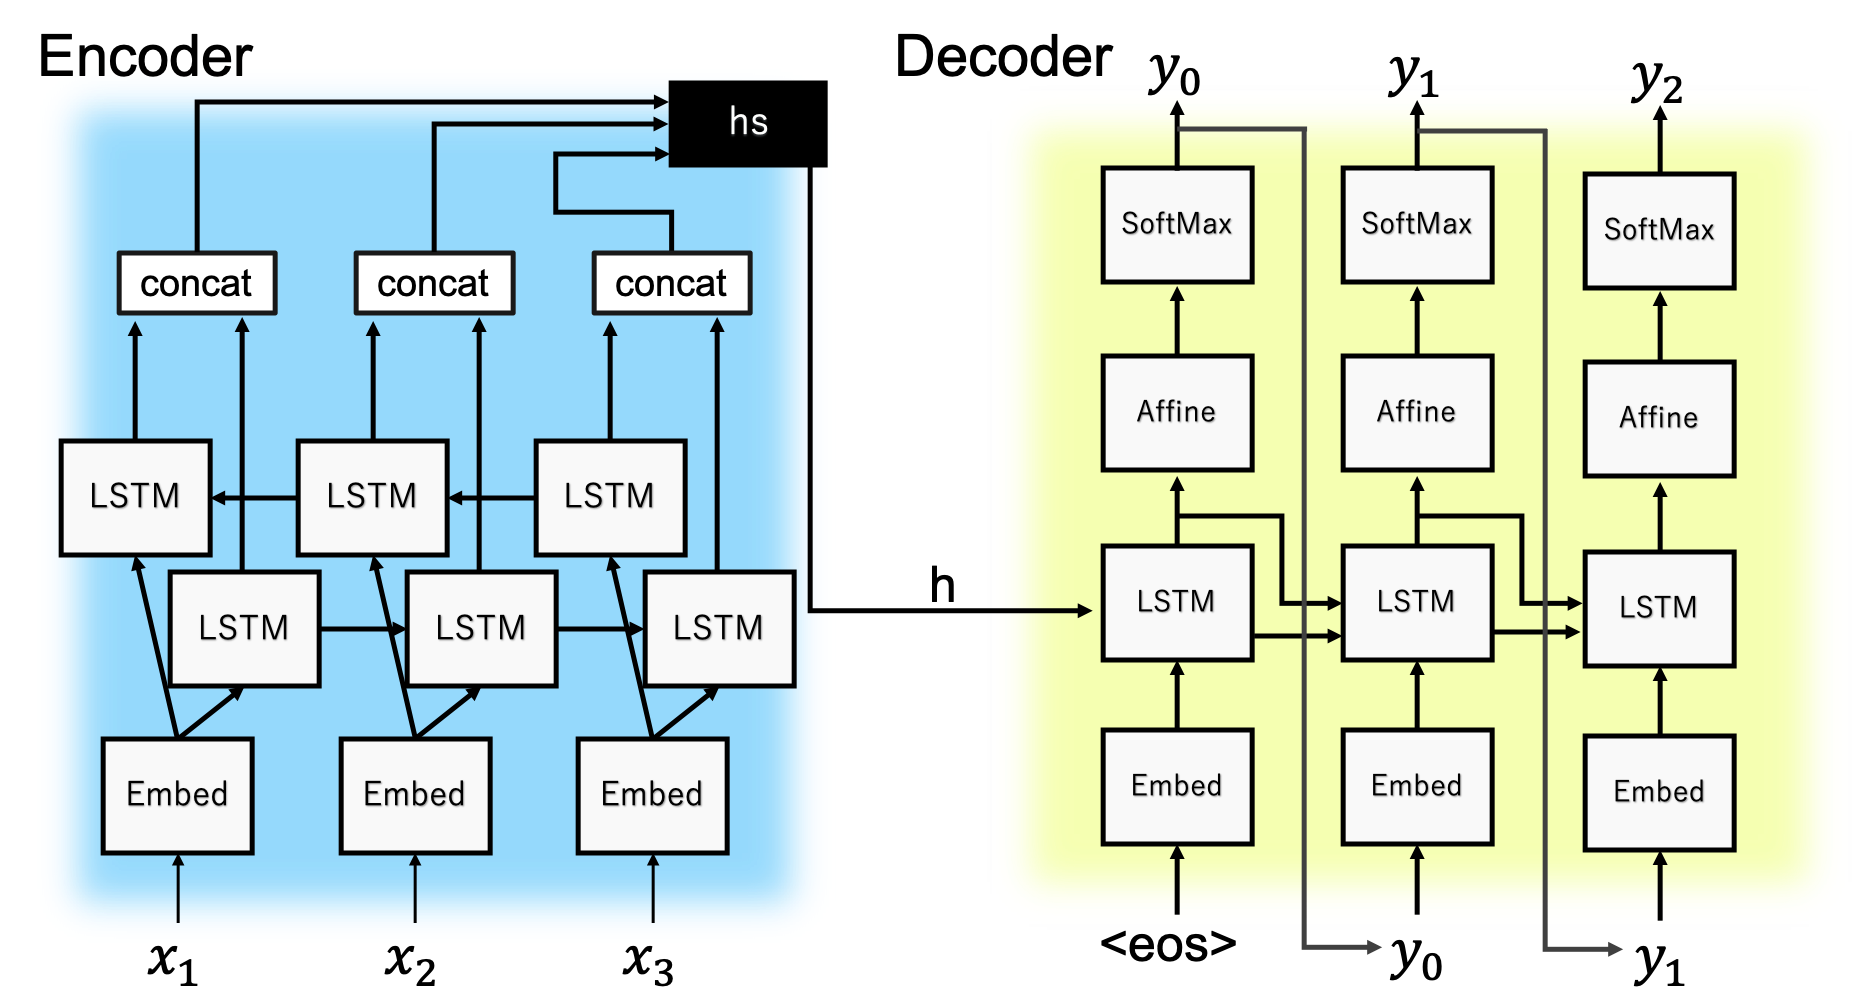
\includegraphics[width=0.9\linewidth]{image/twinRNN.png}
    \caption{bi-directionlモデル}
    \label{fig:Bi-Directional Seq2seq}
  \end{figure}
\end{center}




\chapter{結果とその検討 \label{ch:result}}


\section{実験内容}
以降では今回の実験内容(目的および方法)について説明する.

\subsection{実験1:計算式の特徴量抽出}
\begin{itemize}
  \item 目的.数式のベクトル表現は可能なのかどうか
  \item 方法.埋め込み層,ネットワーク構成を変えながらEncoderの出力値をPCA,t-SNEで二次元ベクトルに圧縮し図示し確認する
\end{itemize}

実験で試したネットワーク構成を表\ref{tb:network_collection}に示す.

\begin{table}[H]
  \centering
  \caption{ネットワーク構成}
  \begingroup
  \scalefont{0.9}
  \begin{tabular}{|l|c|r|r|r|} \hline
    モデル & 入力サイズ & Encoderの出力サイズ & LSTM層の数 \\ \hline \hline
    Normal& 22       & 200              &      1 \\
    &          & 200              &      4 \\
    &          & 200              &      8 \\
    &          & 500              &      1 \\
    &          & 500              &      4 \\
    &          & 500              &      8 \\
    &          & 1000             &      1 \\
    &          & 1000             &      4 \\
    &          & 1000             &      8 \\ \hline \hline
    SkipConnect& 22       & 200              &      1 \\
    &          & 200              &      4 \\
    &          & 200              &      8 \\
    &          & 500              &      1 \\
    &          & 500              &      4 \\
    &          & 500              &      8 \\
    &          & 1000             &      1 \\
    &          & 1000             &      4 \\
    &          & 1000             &      8 \\ \hline \hline
    BiDirectional& 22       & 200 &      1 \\
    &          & 500              &      1 \\
    &          & 1000             &      1 \\ \hline
  \end{tabular}
  \label{tb:network_collection}
  \endgroup
\end{table}

\subsection{実験2:計算式の類題選出}
\begin{itemize}
  \item 目的.数式のベクトル表現は類題選出として利用可能かどうかの検証
  \item 方法.以下の5種類の式に近い式を算出した.
  式の選定基準は一つ目は単純な式,二つ目は分数を含む式,三つ目は小数を含む式,
  四つ目はかっこが含まれる式,五つ目は四つ目のかっこの前の係数だけ変更した式となっている.これらにより類題として選出されるものがどう変化するかを確認した.
  100種類の方程式を表\ref{tb:network_collection}で示したネットワークでベクトル化を行なったのち,学習した式との類似土を計算する.
  算出にはcos類似度を用いて求める.

  \begin{enumerate}
    \item \par \verb#x-3=7#
    \item \par \verb#f{4}{3}x-9=-10#
    \item \par \verb#0.1x=0.5x-1.6#
    \item \par \verb#2(x+5)=6#
    \item \par \verb#-4(x+5)=6#
  \end{enumerate}

\end{itemize}

\section{実験結果}
\subsection{実験1:計算式の特徴量抽出}
学習データ20個を学習し,Encoderの出力の式の分散表現と思われるものの分布である.
学習データの先頭20個を示す.
\begin{itemize}
  \item \par \verb#x+5=8#
  \item \par \verb#5x-7=4#
  \item \par \verb#3.6+x=-1.4#
  \item \par \verb#3x-4=-5x+5#
  \item \par \verb#\frac{7}{2}x+9=6#
  \item \par \verb#3(2x-1)=9#
  \item \par \verb#\frac{3}{7}x+2=\frac{6}{7}#
  \item \par \verb#-\frac{4}{7}x+3=-\frac{1}{7}x#
  \item \par \verb#\frac{x+1}{3}+\frac{2x+1}{2}=\frac{3x-4}{2}#
  \item \par \verb#-4x+9=1#
  \item \par \verb#5x-9=10#
  \item \par \verb#7.2x-4=2.2x+9#
  \item \par \verb#3(x-4)=7x-10#
  \item \par \verb#\frac{3}{7}x-3=-5#
  \item \par \verb#-\frac{9}{8}x-4=-3x#
  \item \par \verb#\frac{x-5}{4}+6=\frac{5}{2}#
  \item \par \verb#\frac{2x+1}{5}=\frac{x-5}{4}#
  \item \par \verb#0.8x-(0.01x-2)=0.03x-2#
  \item \par \verb#-10x-5=8#
  \item \par \verb#5x+10=1#
\end{itemize}

この20個の式を学習させ,pcaを用いて2次元に圧縮し二次元座標平面状にプロットしたものが以下の図\ref{fig:Simple1_200}から\ref{fig:Bi1000layer1}である.

\begin{figure}[htpb]
  \centering
  \begin{tabular}{c}
    \begin{minipage}{0.5\hsize}
      \centering
      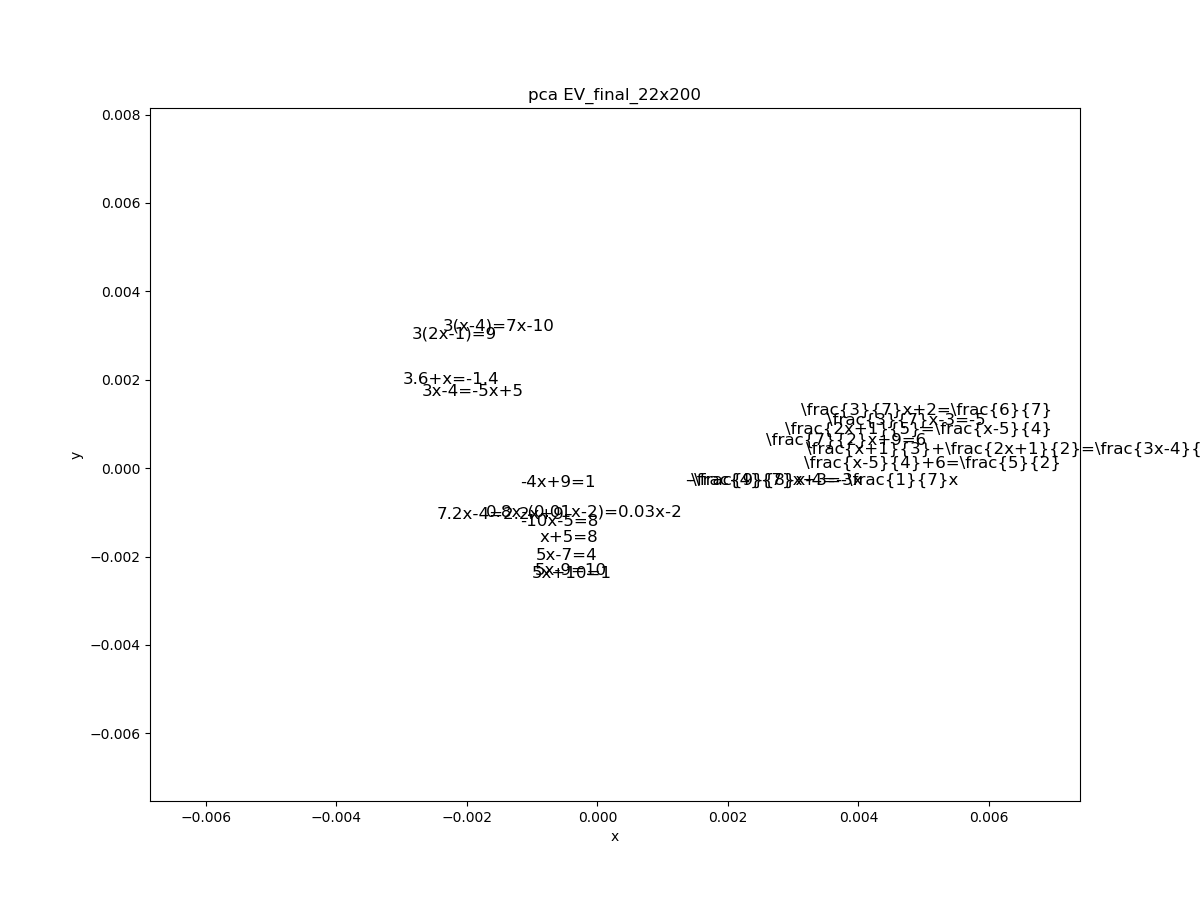
\includegraphics[width=\linewidth]{result/pca_formula_EV_final_22x200_1_Wed_Feb_06_06:17:39.png}
      \caption{Normal LSTM1層200次元 学習データ}
      \label{fig:Simple1_200}
    \end{minipage}

    \begin{minipage}{0.5\hsize}
      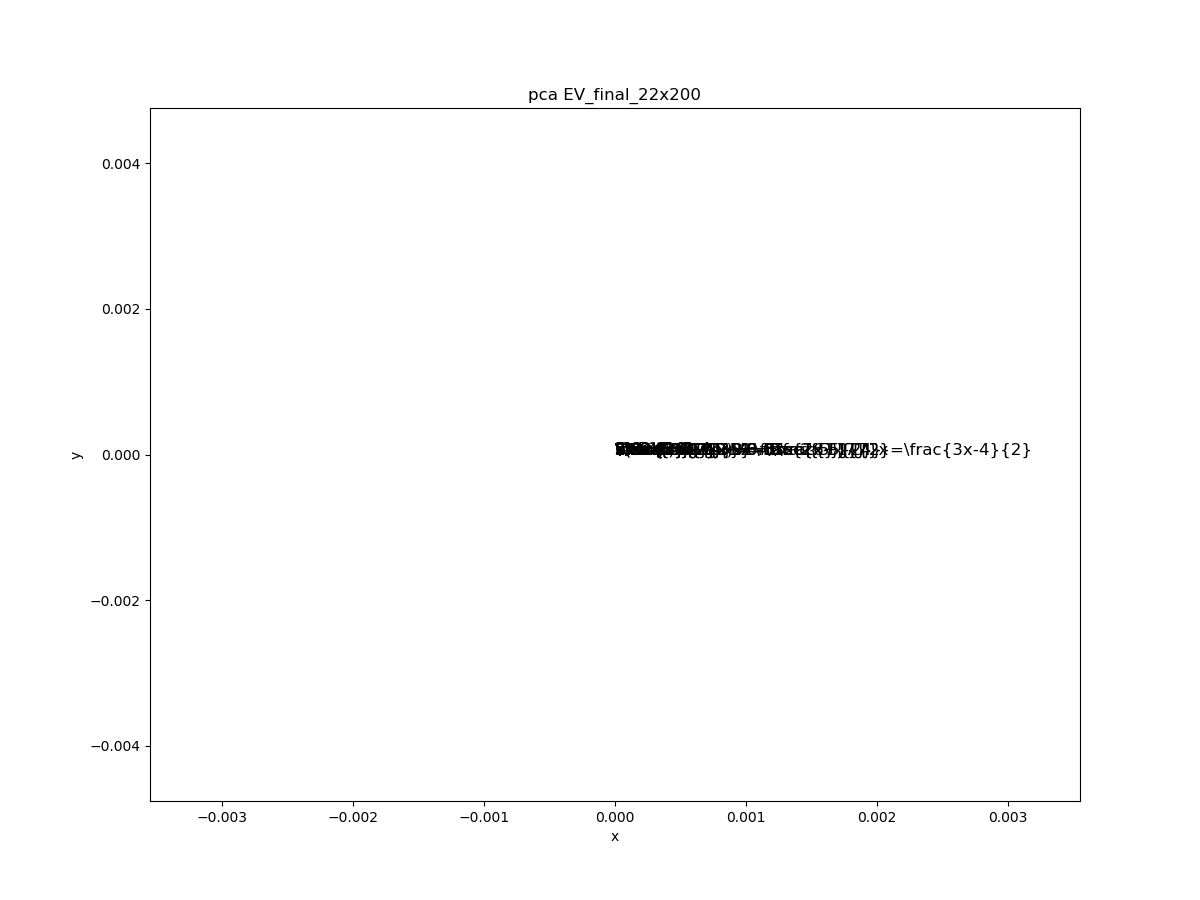
\includegraphics[width=\linewidth]{result/pca_formula_EV_final_22x200_4_Wed_Feb_06_06:19:53.png}
      \caption{Normal LSTM4層200次元 学習データ}
      \label{fig:Simple4_200}
    \end{minipage}
  \end{tabular}

  \begin{tabular}{c}
    \begin{minipage}{0.5\hsize}
      \centering
      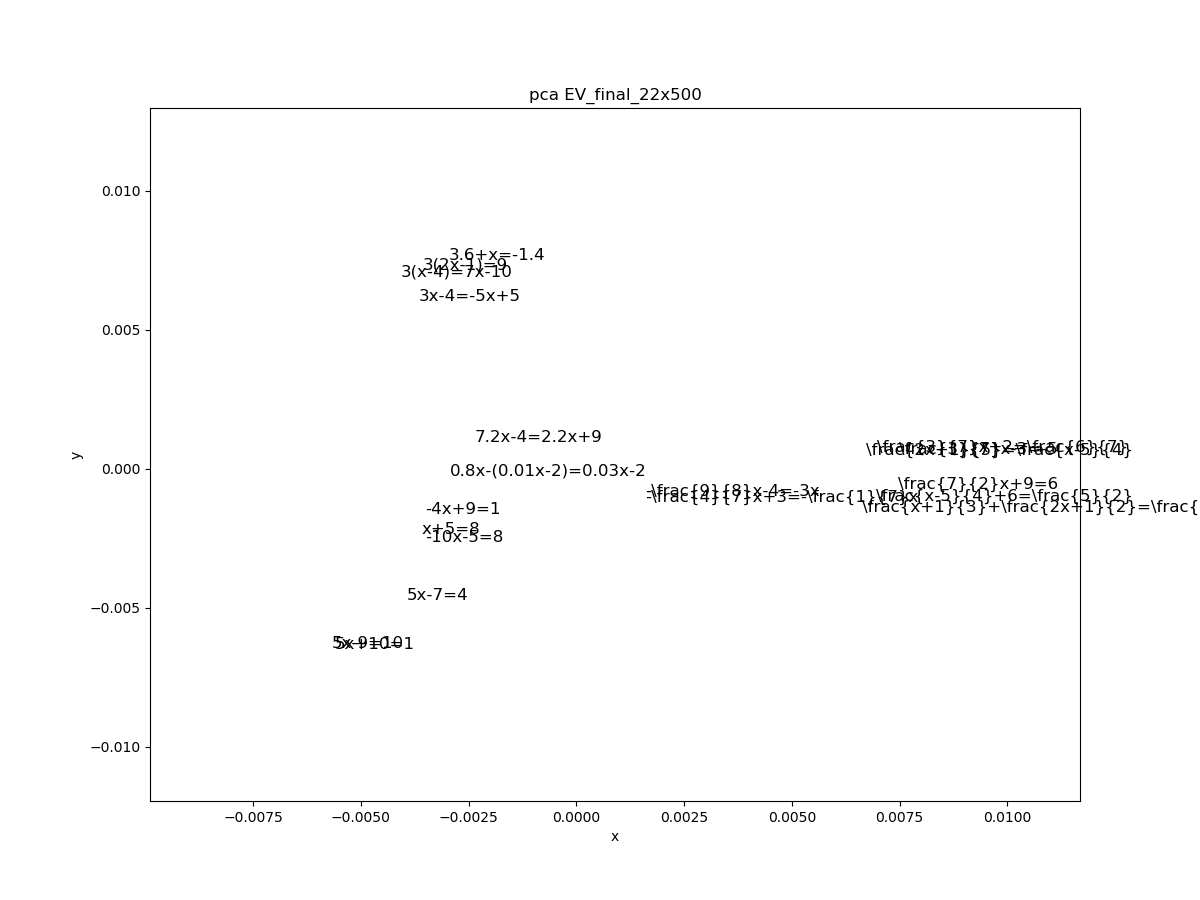
\includegraphics[width=\linewidth]{result/pca_formula_EV_final_22x500_1_Wed_Feb_06_06:28:21.png}
      \caption{Normal LSTM1層500次元 学習データ}
      \label{fig:Simple1_500}
    \end{minipage}

    \begin{minipage}{0.5\hsize}
      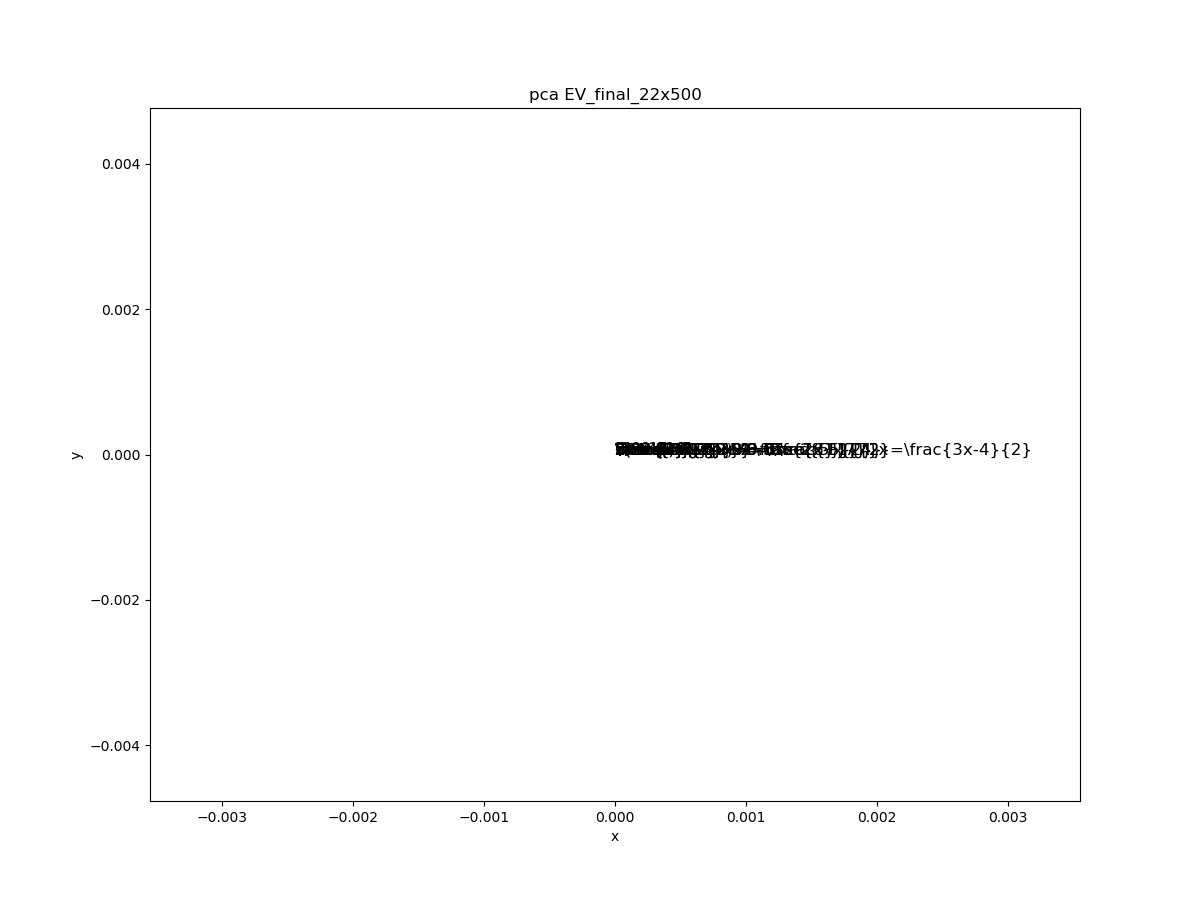
\includegraphics[width=\linewidth]{result/pca_formula_EV_final_22x500_4_Wed_Feb_06_06:43:57.png}
      \caption{Normal LSTM4層500次元 学習データ}
      \label{fig:Simple4_500}
    \end{minipage}

  \end{tabular}
  \label{fig:normal}
\end{figure}



\begin{figure}[htpb]
  \centering
  \begin{tabular}{c}
    \begin{minipage}{0.5\hsize}
      \centering
      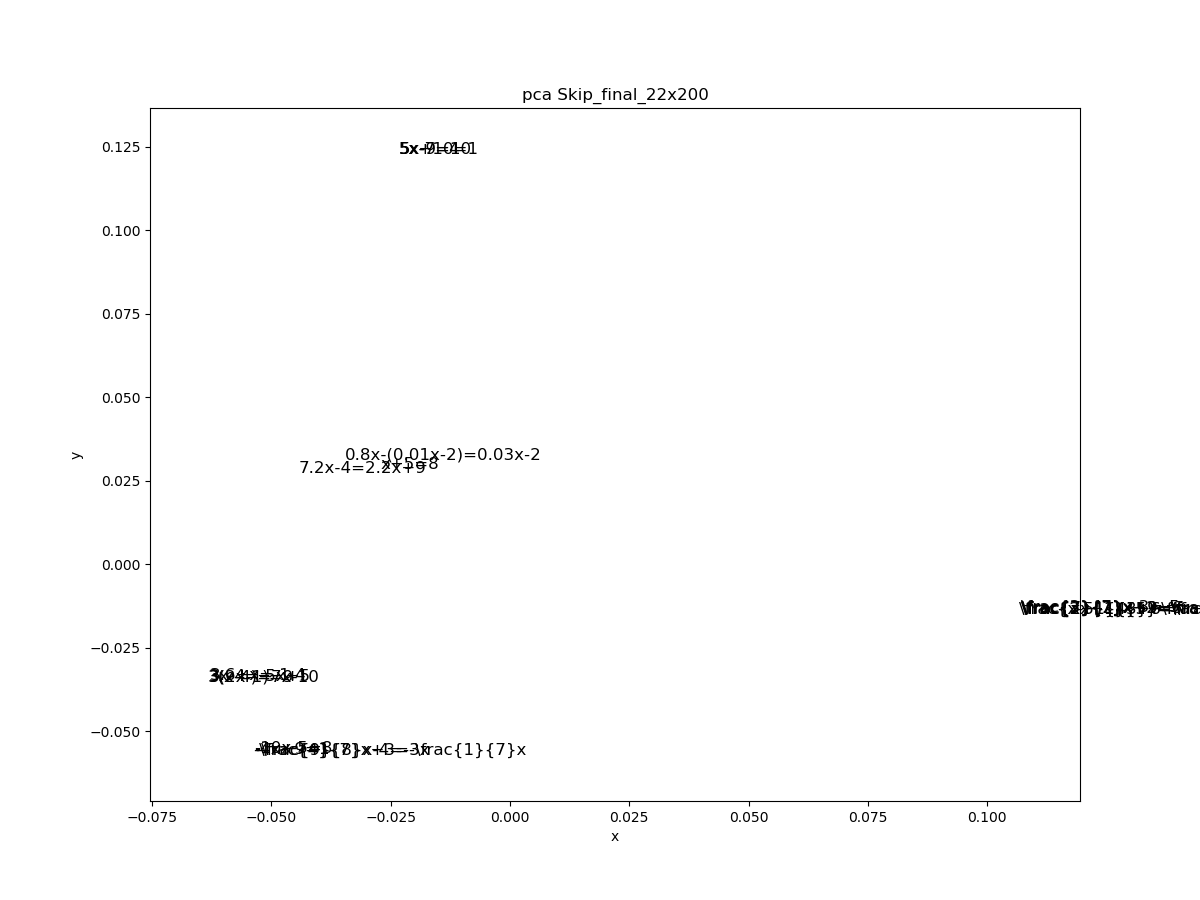
\includegraphics[width=\linewidth]{result/pca_formula_Skip_final_22x200_1_Wed_Feb_06_06:19:41.png}
      \caption{Skipconnect:LSTM1層200次元 学習データ}
      \label{fig:Skip200layer1}
    \end{minipage}

    \begin{minipage}{0.5\hsize}
      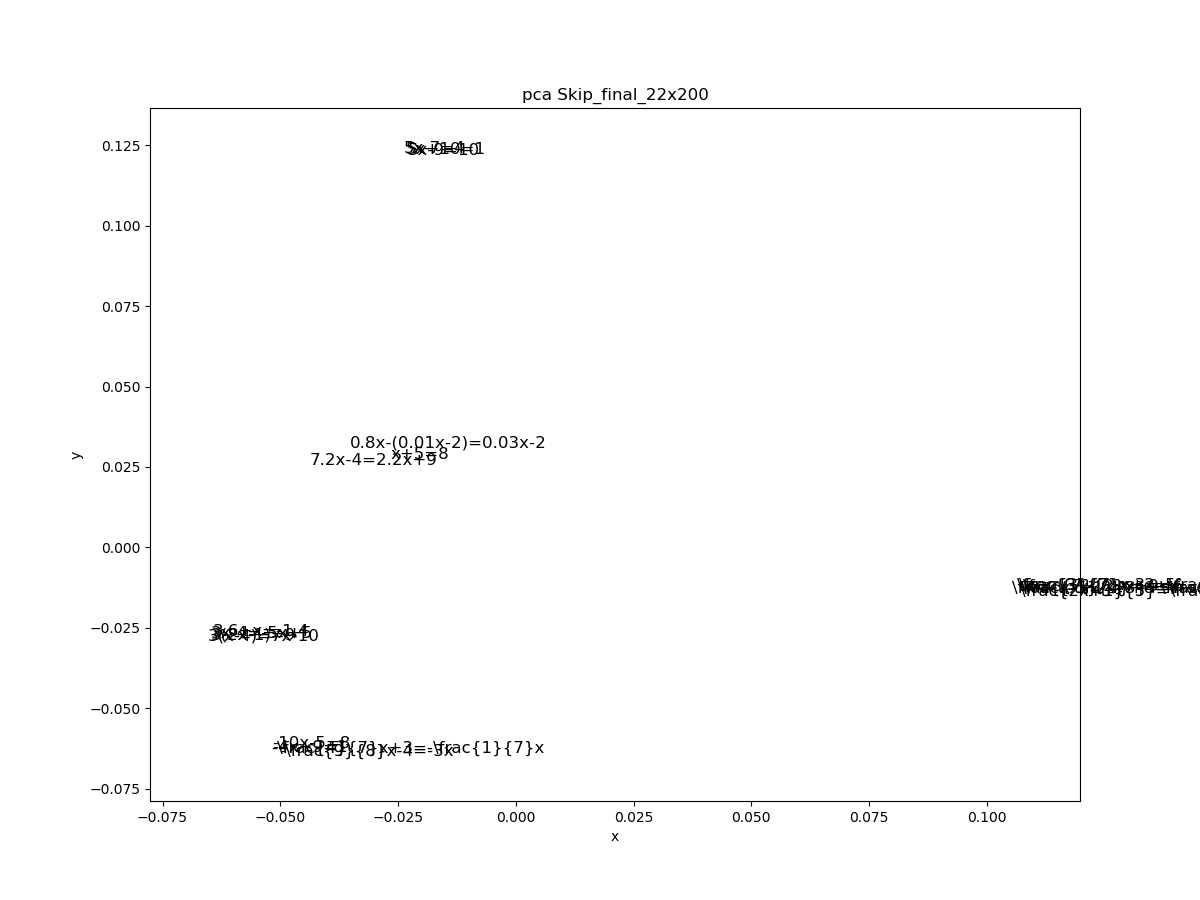
\includegraphics[width=\linewidth]{result/pca_formula_Skip_final_22x200_4_Wed_Feb_06_06:22:39.png}
      \caption{Skipconnect:LSTM4層200次元 学習データ}
      \label{fig:Skip200layer4}
    \end{minipage}

  \end{tabular}

  \begin{tabular}{c}
    \begin{minipage}{0.5\hsize}
      \centering
      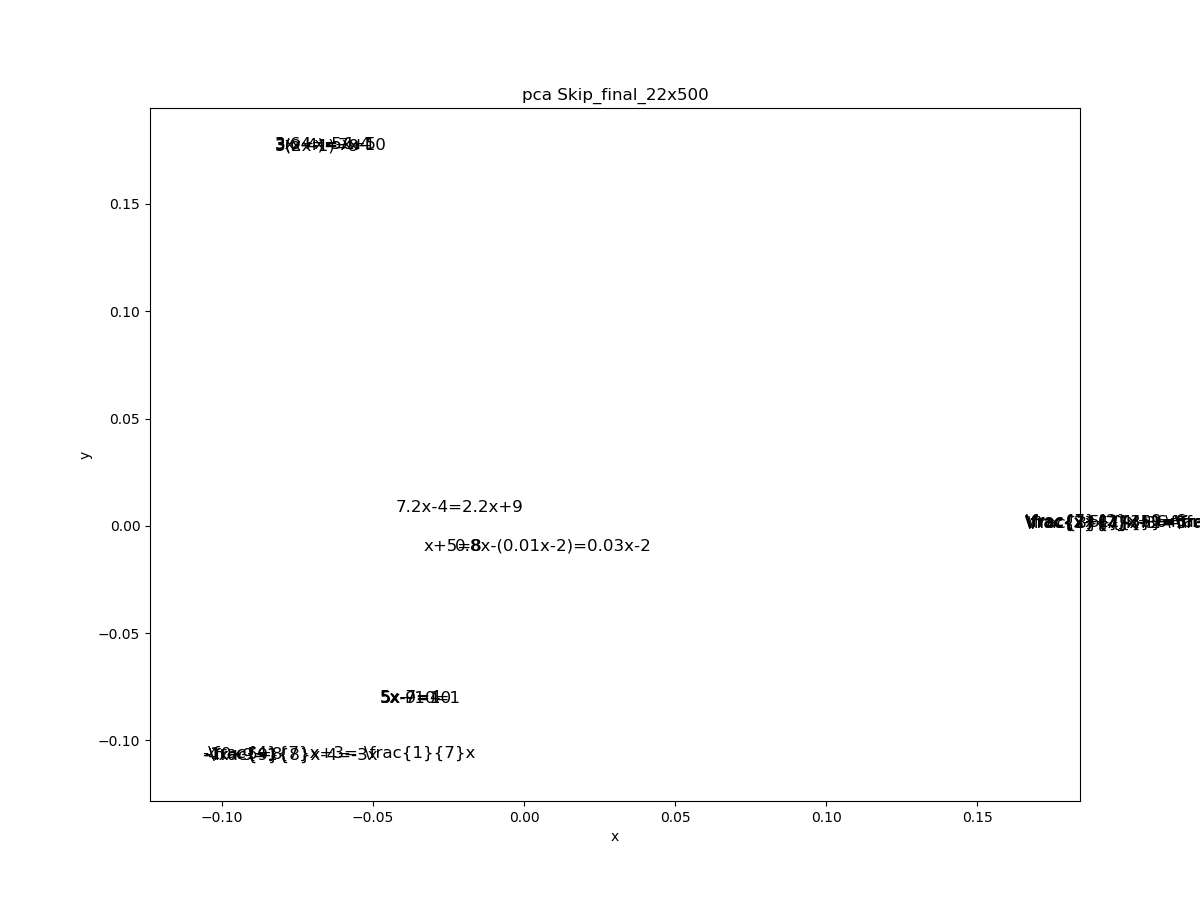
\includegraphics[width=\linewidth]{result/pca_formula_Skip_final_22x500_1_Wed_Feb_06_06:35:09.png}
      \caption{Skipconnect:LSTM1層500次元 学習データ}
      \label{fig:Skip500layer1}
    \end{minipage}

    \begin{minipage}{0.5\hsize}
      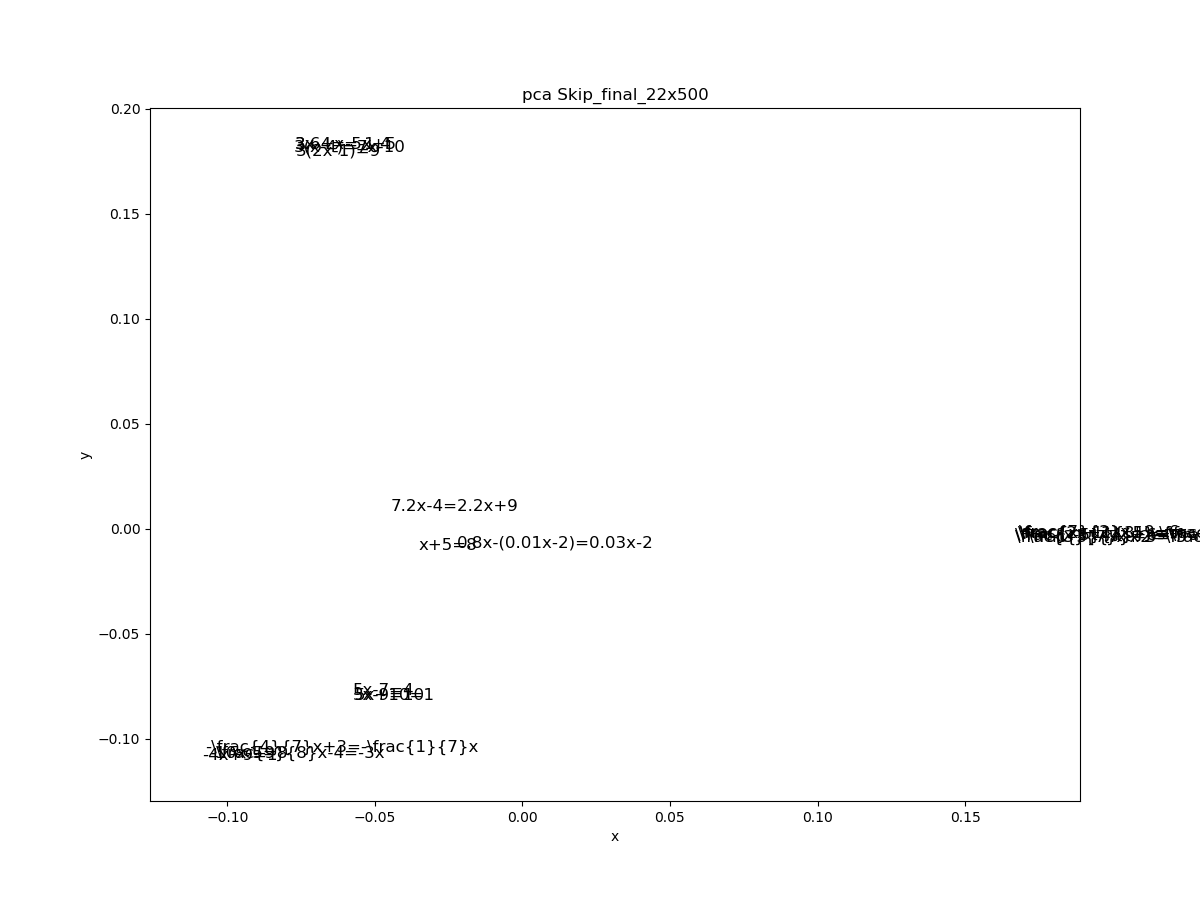
\includegraphics[width=\linewidth]{result/pca_formula_Skip_final_22x500_4_Wed_Feb_06_06:47:59.png}
      \caption{Normal LSTM4層500次元 学習データ}
      \label{fig:Skip500layer4}
    \end{minipage}

  \end{tabular}
  \label{fig:skip}
\end{figure}



\begin{figure}[htpb]
  \centering
  \begin{tabular}{c}
    \begin{minipage}{0.5\hsize}
      \centering
      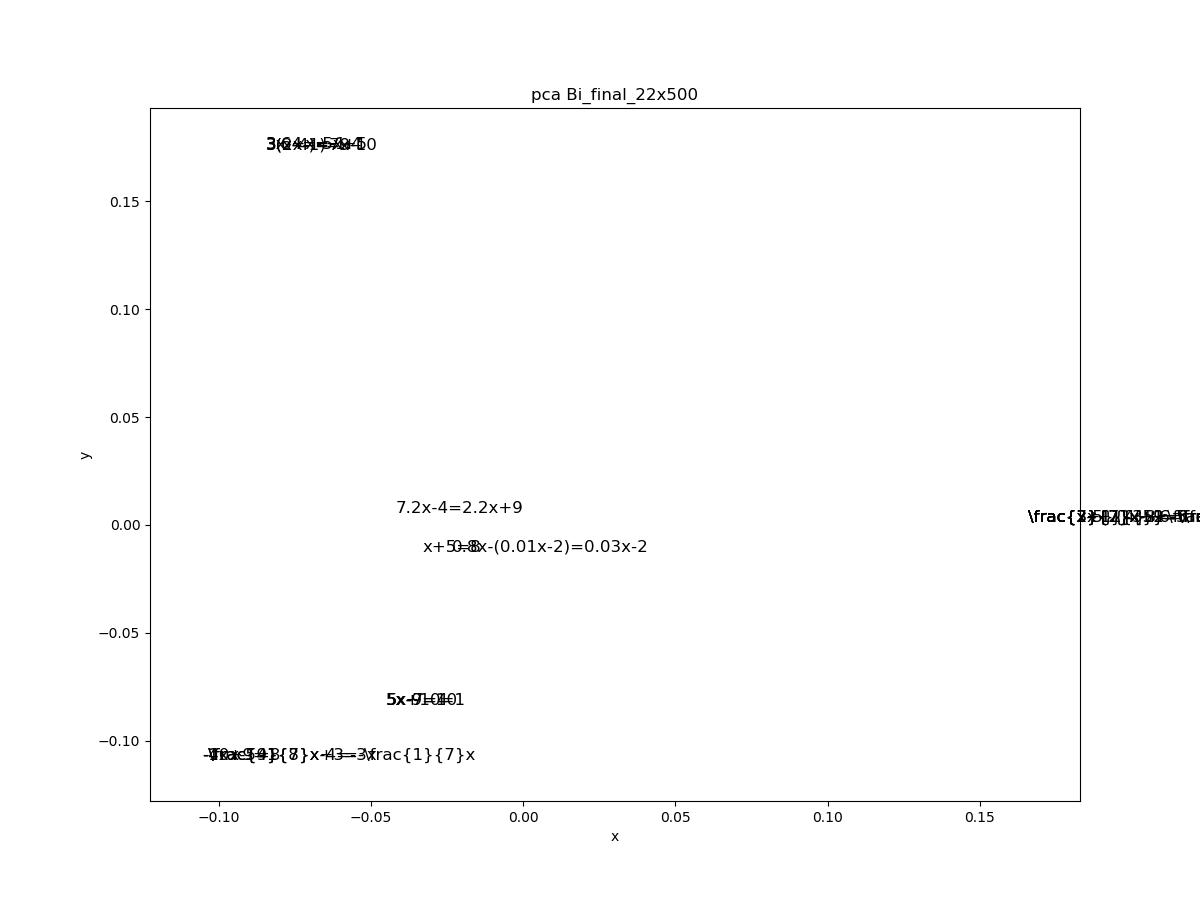
\includegraphics[width=\linewidth]{result/pca_formula_Bi_final_22x500_1_Wed_Feb_06_06:26:57.png}
      \caption{BiDirection:LSTM1層500次元 学習データ}
      \label{fig:Bi500layer1}
    \end{minipage}

    \begin{minipage}{0.5\hsize}
      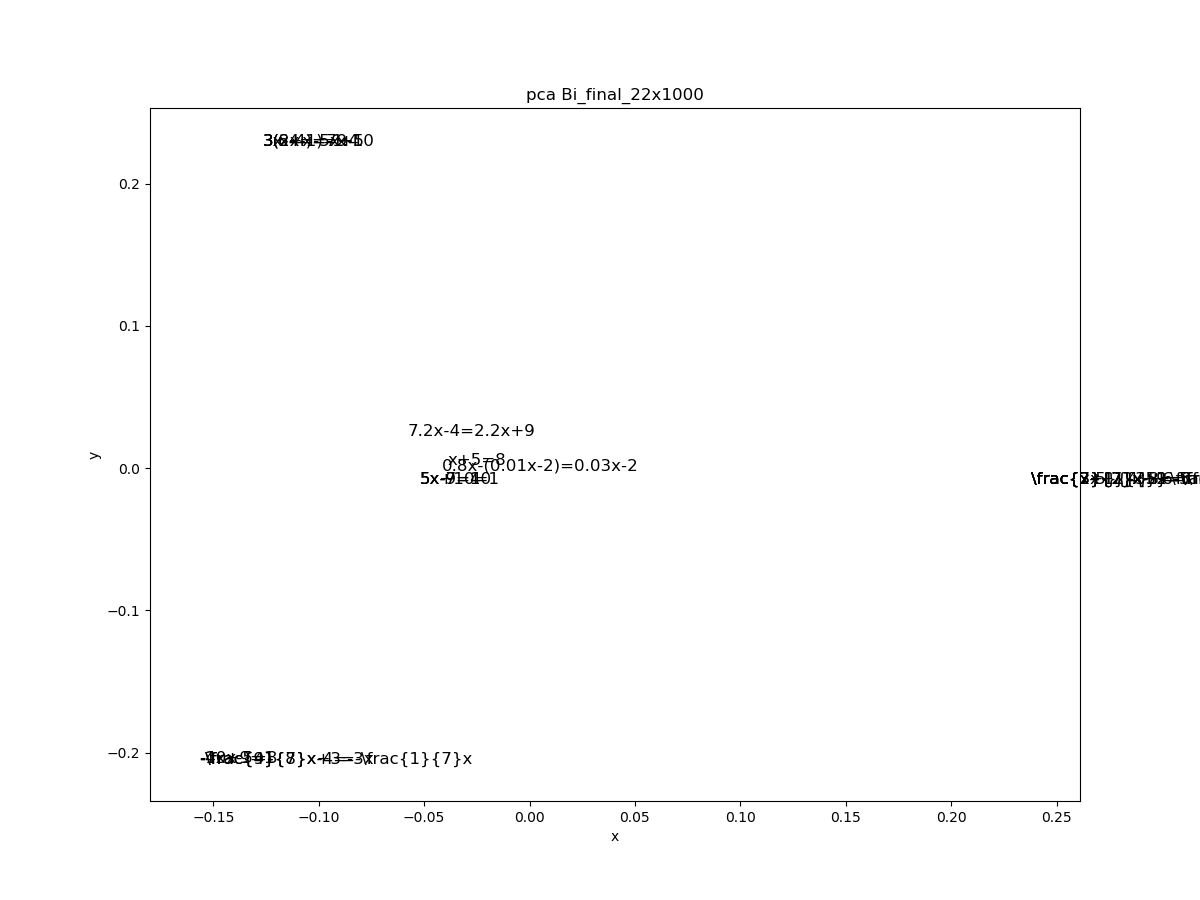
\includegraphics[width=\linewidth]{result/pca_formula_Bi_final_22x1000_1_Wed_Feb_06_06:54:20.png}
      \caption{BiDirection:LSTM1層1000次元 学習データ}
      \label{fig:Bi1000layer1}
    \end{minipage}
  \end{tabular}
  \label{fig:Bi}
\end{figure}


\clearpage
\subsection{実験2:計算式の類題選出}
表\ref{tb:network_collection}で示したネットワークごとに並べている.冒頭に
(学習ネットワーク方法,次元数,LSTM層の層数)で学習方法を示している,
全ての結果は付録\ref{ch:sub}に掲載する.各モデルの$-4(x+5)=6$の実行結果である.

\verbatimtabinput[3]{-4(x+5).log}
\clearpage

\section{考察}

\subsection{実験1:計算式の特徴量抽出について}
今回の実験ではNormalEncoder,SkipConnection,BiDirectionalの三種類のEncoderについて評価実験を行った.
NormalEncoderでも200次元では分布として分かれていたが,LSTMを深くすると勾配が消失し,一点に集中している(図\ref{fig:Simple4_200},図\ref{fig:Simple4_500}).
しかし,図\ref{fig:Simple4_200}と図\ref{fig:Skip200layer4},図\ref{fig:Simple4_500}と図\ref{fig:Skip500layer4}を比較してみると
SkipConnectionを用いることで多層LSTMで学習しても過学習が発生することを防ぐ事が確認できた.

またBi-Directionalではテストデータでも高精度に分類できており,それぞれのencoderの効果がみて取れた.

図\ref{fig:normal},図\ref{fig:skip},図\ref{fig:Bi}のどれもが同系列そうな問題が近い分布となった.
図\ref{fig:Simple1_200}ですらは分数の中でも符号でも分かれており,拡大してみてみると式の始まりが負の方程式だけまとまっているところがありわずかながらその違いを表しているように見える(図\ref{fig:normal200cut}).


\begin{center}
  \begin{figure}[H]
    \centering
    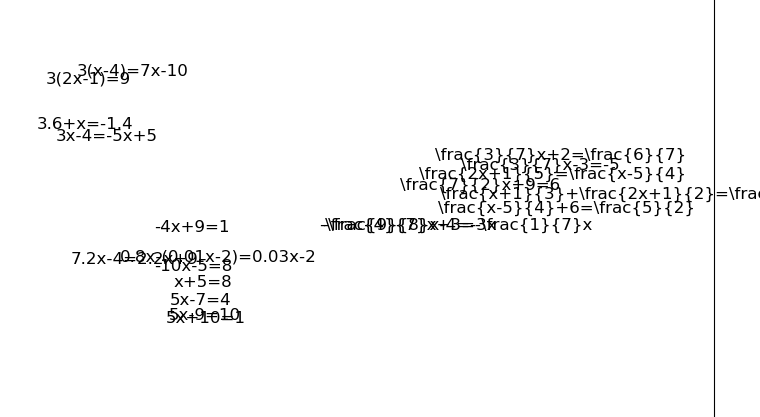
\includegraphics[width=\linewidth]{image/detial/pca_formula_EV_final_22x200_1_cut.png}
    \caption{NormalRNNで作った200次元のExericisesVecterの一部}
    \label{fig:normal200cut}
  \end{figure}
\end{center}

特に図\ref{fig:Bi500cut2}と図\ref{fig:Bi1000cut}をみるとBi-DirectionalRNNで作った500次元のExericisesVecterの方が
小数を含む式と整数だけの式の距離がより離れ,分類がより正確になっているように見える.
このことからより高次元で再構成すると高い再現率が得られるとは言えず.繊細なチューニングが不可欠である.

\begin{center}
  \begin{figure}[H]
    \centering
    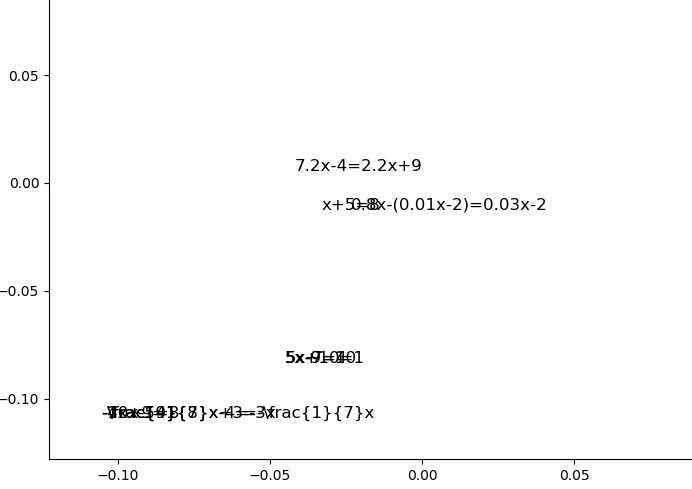
\includegraphics[width=\linewidth]{image/detial/pca_formula_Bi_final_22x500_1_cut.png}
    \caption{Bi-DirectionalRNNで作った500次元のExericisesVecterの一部}
    \label{fig:Bi500cut2}
  \end{figure}
\end{center}


\begin{center}
  \begin{figure}[H]
    \centering
    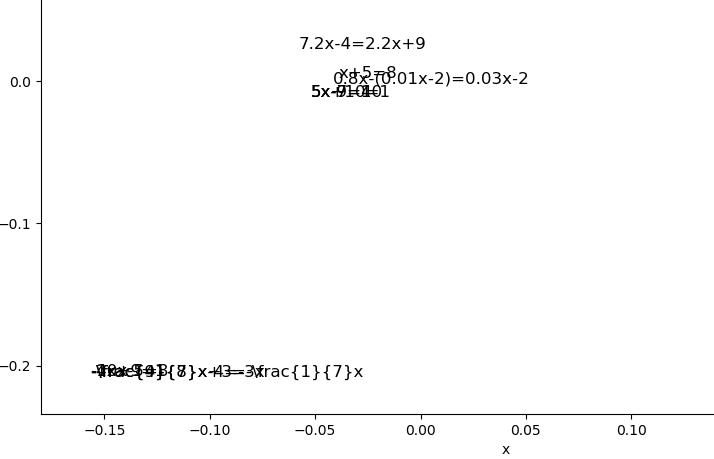
\includegraphics[width=\linewidth]{image/detial/pca_formula_Bi_final_22x1000_1_cut0.png}
    \caption{Bi-DirectionalRNNで作った1000次元のExericisesVecterの一部}
    \label{fig:Bi1000cut}
  \end{figure}
\end{center}




このことより系列変換を用いて数式の分類は可能であり応用の余地がある事が確認できた.
ただし,SkipConnectでは層を深くしても過学習は起こらないが特徴をうまく捉え切ることができなかった.

\subsection{実験2:計算式の類題選出}

どのモデルパターンも単純な$x-3=7$は同じような式が類似度トップ5に並んでいる.
各モデルパターンでは次元数の200,500,1000では類似度に違いはあっても選出される式に違いはなかった.

$-4(x+5)=6$はネットワークごとに違いが出ておりnormalの500次元1層やSkipConnectの500次元4層ではカッコを使った式の出現は少ないもののBi-Directional200次元一層ではカッコがあるものが8割を占めており,何らかの特徴を抽出できているのではないかと考える.
この結果から式の特徴抽出には双方向RNNが有効であることがわかる.



\chapter{関連研究\label{ch:relsatedwork}}
自然言語処理を数式を適用した例は筆者が調べるかぎりは存在しない.
自然言語以外にWord2vecを適用しようとした研究はいくつかある.
文献\cite{kannrenn3}では文の特徴をEncoder-Decoderの機構を用いて学習し,本研究と同様にEncoderの隠れ層の出力により文章の類似度を算出している.文献\cite{kannrenn3}によると小説の一部を学習データに用いて,埋め込み層としてSkipGramを適用している.gensimのDoc2Vecとの比較がなされているが,ユーザにとって有益な評価方法の設定の難しさを述べている.
これらの文章をベクトル化するというのは文献\cite{1612.06778}から始まり注目を集めている.

\begin{center}
  \begin{figure}[H]
    \centering
    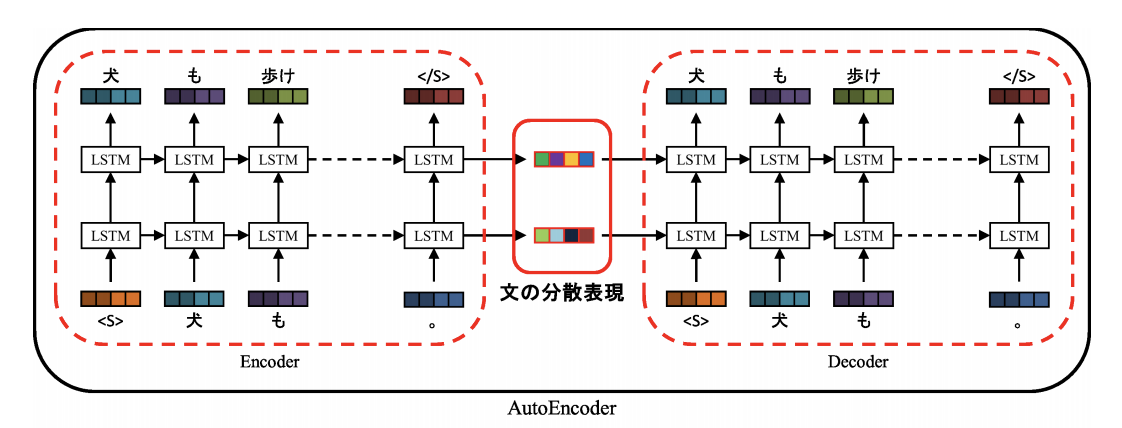
\includegraphics[width=\linewidth]{image/lstm_hidden_vecter.png}
    \caption{文献\cite{kannrenn3} ネットワーク構成}
    \label{fig:kannrenn3fig}
  \end{figure}
\end{center}

文献\cite{lannrenn4}ではエラーのあるプログラムコードを埋め込み,再構成して実行できるプログラムを再構成できるか試している.C言語で書かれたプログラムを一文字ごと,onehot化して読み込んでいる.この論文では大小文字を区別して学習する.1-D Convolutionを用いて情報を圧縮し再構成することで上記のことが可能だと述べている.Dropoutを用いると性能が向上しており,自然言語と同様に過学習が通常のRNNでは起きるので,対策として本論文でもDropoutを採用した.

文献\cite{kannrenn5}ではDeepLearingの技術の検索の際,ユーザが求めている情報を推奨することを目的としている.
評価方法としてMovie Lens-100Kでの映画の推奨をパラメータ,ネットワークの構成を様々試しながら知見を集めている.
AutoEncoderは層を重ねても,性能は向上せず,各映画のユーザ平均を差し引いて正規化しても性能は大きく変化しない.
これにより,特徴抽出の重要さを筆者は述べている.

文献\cite{glyce}は漢字などの象形文字から文字の分散表現を得る研究である.
図\ref{fig:kannji1}で示すように,画像データを畳み込みニューラルネットを持ちいて次元圧縮していき,
最後には1024次元のベクトルとして出力する.この最終層の出力を漢字の分散表現としてもちいて他の自然言語タスクを従来方法より超える結果を出している.特徴として漢字を現在使われている字体だけでなく,旧字体も用いて性能向上を図っている(図\ref{fig:kannji2}).





\begin{center}
  \begin{figure}[H]
    \centering
    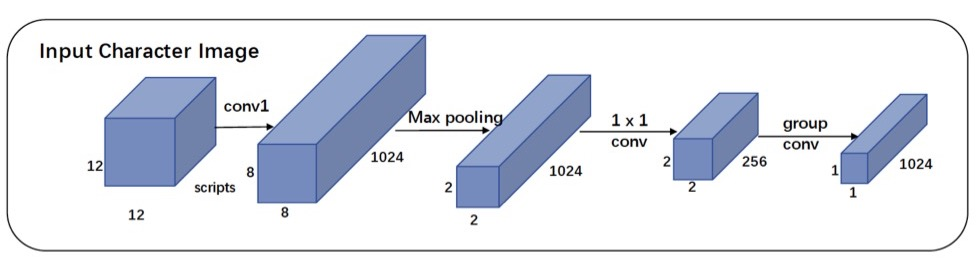
\includegraphics[width=\linewidth]{image/kannji1.jpeg}
    \caption{文献\cite{glyce} ネットワーク構成}
    \label{fig:kannji1}
  \end{figure}
\end{center}



\begin{center}
  \begin{figure}[H]
    \centering
    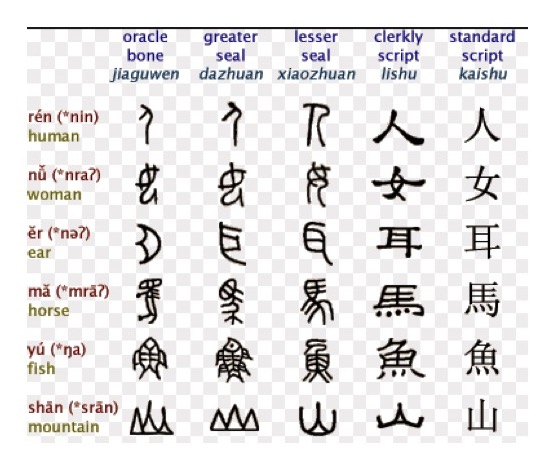
\includegraphics[width=\linewidth]{image/kannji2.jpeg}
    \caption{象形文字も学習に使い,その文字がどのように変化してきたのかも考慮する}
    \label{fig:kannji2}
  \end{figure}
\end{center}




\chapter{結論と今後の課題 \label{ch:conclusion}}
\if0
\point{
序論で提起した問いとそれに対する答えをまとめる.
\begin{itemize}
  \item 提案手法のアイデアおよび評価結果を振り返る.
  \item この研究で得られた知見をまとめる.
  \item 今後の課題について述べる.
\end{itemize}
}
\fi

本研究では自然言語処理の技術を人工言語の数式に適用し,分類ができるかどうかを目的とした.
分散表現で文字の特徴量を抽出したのち,その特徴量を用いて数式の分散表現化を行い,式のベクトルを得た.この結果から現在では間違った問題から人をグループ化していたシステムから問題をグループ化してその問題を間違えた人の最適化学習支援を行い,より繊細で効果的な学習が期待できる.
この研究の先には大量の個人情報を扱うアダプティブラーニングにおいて問題から分類できるようになれば,学習データが少なくても十分に効果を発揮することが期待できる.

これにより数式データのみで最適な問題選択を可能とし,いまある個人情報と合わせるとより高い精度でシステムが提供できるように思う.
これは人間が作り発展させてきたものはどこか本質的には同様の特徴を持っており,その特徴をコンピュータが学ぶことができるということではないだろうか.

しかしながら,未だ問題点はある.
計算問題には優しい問題ほどパターンがなくなり,式から有用な情報が取り出せなくなる.
また,多くの子供が苦手とする文章題は本研究では扱っていないが,Doc2Vecなど文章をベクトル化する手法は提案されており,それを応用することにより可能性は広がるだろう.
本研究で扱った一次方程式の特徴量を使って別の分野に転移学習を行うとより,
包括的なアダプティブラーニングシステムの構築が行えるようになることを期待している.



\appendix

\chapter{実験2:計算式の類題選出の実行結果\label{ch:sub}}
\if0
\begin{itemize}
  \item 文字コードはUTF-8に統一する.
  \item 論文ファイル名は\texttt{chishiro-thesis.tex},文献ファイル名は\texttt{chishiro.bib}のように名前\texttt{-thesis.tex}とする.
  \item 句読点は全角のカンマ,ピリオドを用いる.
  \item 英数字はすべて半角を用いる.ギリシャ文字は{\TeX}の定義を用いる.$\alpha, \beta, ...$
  \item カンマの前にはスペースを入れず,カンマの後はスペースをひとつ入れる.
  \item 数式は{\TeX}の数式機能を用いる.例: $x^2$,\[f(x) = x^2 + 2x + 1.\].
  \item プログラムテキストはタイプライターフォントを用いる(例: \texttt{hello}).
  \item 文章構成(章・節・小節・箇条書き)は{\TeX}の機能を用いて指定する.自分で見出しなどを作らない.
  \item 題目には研究目的・方法・対象を特徴づける情報を入れる.
  \item 図のタイトルは図の下,表のタイトルは表の上に書く.
  \item 図表番号の参照は\verb#\label#および\verb#\ref#を用いる.自分で図表番号を指定しない.
  \item 表は{\TeX},グラフはすべてpythonで作成する.
  \item 図表番号のない図は用いない.
  \item 参照の?は必ず取り除く.
  \item 段落は意味の区切りでわける.意図しない字下げが入った場合\verb#\noindent#を用いて修正する.
  \item 参考文献は10以上あげる.
\end{itemize}
\fi




\verbatimtabinput[3]{txt/E2D200_1.log}
\verbatimtabinput[3]{txt/E2D200_4.log}

\verbatimtabinput[3]{txt/E2D200_8.log}
\verbatimtabinput[3]{txt/E2D500_1.log}

\verbatimtabinput[3]{txt/E2D500_4.log}
\verbatimtabinput[3]{txt/E2D500_8.log}

\verbatimtabinput[3]{txt/E2D1000_1.log}
\verbatimtabinput[3]{txt/E2D1000_4.log}

\verbatimtabinput[3]{txt/E2D1000_8.log}
\verbatimtabinput[3]{txt/similerskip200_1.log}

\verbatimtabinput[3]{txt/similerskip200_4.log}
\verbatimtabinput[3]{txt/similerskip200_8.log}

\verbatimtabinput[3]{txt/similerskip500_1.log}
\verbatimtabinput[3]{txt/similerskip500_4.log}

\verbatimtabinput[3]{txt/similerskip500_8.log}
\verbatimtabinput[3]{txt/skip1000_1.log}

\verbatimtabinput[3]{txt/skip1000_4.log}
\verbatimtabinput[3]{txt/skip1000_8.log}

\verbatimtabinput[3]{txt/Bi200_1.log}
\verbatimtabinput[3]{txt/Bi500_1.log}

\verbatimtabinput[3]{txt/Bi1000_1.log}


\bibliography{miyaji}


\chapter*{謝辞 \label{ch:acknowledgement}}
\thispagestyle{empty}
\if
\point{
本のあとがきに相当する部分.半ページ 以上書く.
卒業研究に協力者してくれた方々へのお礼を忘れずに述べる.
}
\fi
この研究を進めるにあたって,私の興味の赴くまま進める中,様々な角度からご指導いただいた千代教授に深く感謝申し上げます.
また研究が行き詰まると,会話を通して気づきを与えてくれた同研究室メンバーに感謝申し上げます.
そしてこの研究では自然言語処理の奥深さをただただ感じました.そんな時,常に参考になり研究の日々を共に過ごしたゼロから作るDeepLearning 2 自然言語処理編\cite{ZeroDeep}には山ほど助けられました.
Pythonからscalaに書き換えながら理解を進めることができ芯から理解することができたように思います.

最後に,毎週たくさんの計算問題を宿題として解いてきてくれた私の塾の生徒たちに心から感謝と未来の活躍を祈るとともに
必ず,この経験を糧に世の中により良い教育システムを提供し今まで手の届かなかった子供達の未来に手助けすることを約束し,謝辞といたします.


\end{document}
